\documentclass{article}
\usepackage{inc}

\usepackage{geometry}
 \geometry{
 a4paper,
 total={170mm,257mm},
 left=20mm,
 top=20mm,
 }

\title{Rapport de stage -- Introduction à la théorie des catégories}
\author{Aurélien VANDEWEYER}
\date{Avril 2023}

\begin{document}
\maketitle
\newpage
\tableofcontents
\newpage

\section{Introduction}
\subsection{Introduction au sujet}

L'intention initiale du stage proposé était de fournir un aperçu introductif à la théorie des catégories (TC), une branche des mathématiques qui n'a pas réellement de précédent si ce n'est, comme toujours en mathématiques, de permettre des classifications et généralisations de concepts en les rendant plus abstraits et, par conséquent, plus universelles et plus unificateurs. Les applications de la TC, malheureusement, ne sont pas évidentes à trouver dans la vie réelle, bien qu'il en existe. Pour donner un exemple de l'étendue du sujet, pensons à la théorie des groupes. La théorie des groupes possède des applications intelligibles à partir du moment où l'objet de notre étude possède une quelconque symétrie. Dans la vie de tous les jours, les symétries sont présentes en nombre et la théorie des groupes fournis donc un formalisme pour les étudier, les classifier et finalement unifier les notions communes à tout ce qui possède des symétries.\\

La théorie des catégories est de nature plus profonde. Tout comme la théorie des groupes (ou beaucoup d'autres théories mathématiques), l'idée de sa mise en oeuvre est venue de la forte intuition qu'il existe des concepts, en mathématiques, possédant des "schéma"/"patterns" similaires, mais appliqués à des objets pourtant différents. Nous pouvons donner un exemple rapide motivant cette intuition, nous y reviendrons de toute façon plus en détail le moment venu : en théorie des ensembles, un produit Cartésien consiste à former un ensemble de paires (ordonnées) à partir de deux ensembles initiaux. En logique, une conjonction est une opération permettant de lier deux propositions afin d'en obtenir une nouvelle. En théorie des types (ou en informatique de manière plus générale), un tuple (ou "2-uplet" ou "type produit") permet de combiner deux types en une seule paire. Ces trois exemples, tirés de domaines et de structures différents, ont pourtant en commun cette propriété de "combiner" deux éléments pour en obtenir un nouveau, mais dont les constituants ne sont pas "détruits" et toujours accessibles. Ils semblent être issus d'un même modèle, d'un même schéma qui a été simplement appliqué à différents types d'objets.\\

La théorie des catégories peut donc se résumer comme proposant l'unification de concepts qui semblent éloignés de par les objets auxquels ils s'appliquent, mais universels de par leurs propriétés. L'étude principale de la TC n'est d'ailleurs pas les objets en tant que tels, mais plutôt les relations et les propriétés qui existent entre ces derniers.\\

Historiquement, la théorie des catégories est une théorie générale des structures mathématiques et de leurs relations qui a été introduite par Samuel Eilenberg et Saunders Mac Lane au milieu du XX$^e$ siècle dans leurs travaux fondamentaux sur la topologie algébrique. De nos jours, la théorie des catégories est utilisée dans presque tous les domaines des mathématiques et dans de nombreux domaines de l'informatique.

\subsection{Objectifs du stage}

Durant ce stage, il a été proposé, dans un premier temps, d'explorer les concepts importants de la théorie des catégories et d'introduire les notions de bases telles que les catégories, bien sûr, mais aussi les foncteurs, les épimorphismes, monomorphismes, objets initiaux et terminaux, produit, co-produit, propriété universelle, limites et co-limites, monades et adjoints. Le but du stage était de voir, démontrer et comprendre le lemme de Yoneda, probablement le résultat le plus important en théorie des catégories. Au cours du projet, il a également été proposé de résoudre divers exercices sur les concepts proposés ainsi que des applications aux objets mathématiques déjà connus (comme les ensembles, les groupes ou les anneaux).\\

Dans ce rapport de stage, je présenterai les différents concepts que j'ai appris durant la semaine. J'organiserai ce rapport d'une façon suffisante à lui-même en introduisant les notions à un lecteur supposé ignorant ce qu'est la théorie des catégories, mais possédant des compétences suffisantes en mathématiques, en informatique et en physique. J'insistais sur les notions qui m'ont personnellement posés plus de soucis et j'expliquerai les sujets comme j'aurais aimé qu'ils me soient enseignés.

\subsection{Motivation personnelle}

Bien avant ce stage, je connaissais déjà de nom et de potentiel la théorie des catégories. J'en avais entendu parler dans le contexte de l'informatique théorique, ainsi que dans certains langages de programmation déclaratifs où les concepts catégoriels apparaissent de manière presque inhérente, citons par exemple le langage fonctionnel Haskell, où les monades et les foncteurs sont au coeurs de la conception de programmes, ou encore le langage concaténatif Joy, où la syntaxe correspond à un monoïde libre et la sémantique à un homomorphisme monoïdale (plus simplement, un programme en Joy consiste en une longue composition de sous-programmes et de fonctions).\\

Par moi même, j'aurais de toute façon fini par étudier la théorie des catégories; que ce sujet ait été proposé pour un stage fut donc une bonne occasion pour commencer son exploration, qui plus est dans une ambiante encadrée.

\subsection{Remerciements}
Je souhaite remercier Mattia Serrani, mon promoteur durant cette semaine de stage, pour m'avoir permis d'étudier les bases de la théorie des catégories, de m'avoir orienté, conseillé et enseigné les éléments clefs du sujet. Je le remercie également pour ses relectures (rapport, exercices et poster).

\subsection{A l'intention du lecteur}
Ce rapport de stage comporte très probablement des erreurs et des coquilles (peut-être principalement dans la dernière section, sur le lemme de Yoneda, qui n'a pu être étudié que durant un laps de temps un peu trop court). Le but du \textit{projet personnel} de physique organisé par le département de physique de l'université de Mons était d'initier à la recherche et à la découverte de nouveaux domaines, pas de fournir un travail digne d'une publication. Cela dit, ce travail illustre \textit{à priori} correctement les notions abordées et a déjà été repris quelques fois pour initier à la théorie des catégories par certains assistants du département de physique.

\newpage
\section{Rappels utiles et diagrammes commutatifs}
L'étude de la théorie des catégories, étonnamment, ne demande pas une quantité de pré-requis considérable, en réalité son étude demande plutôt un effort conceptuel et d'abstraction. Tout de fois, certaines notions qui seront constamment utilisées dans la suite se doivent d'être rappelées. Nous allons ici présenter de brèves notions qui seront utiles à garder à l'espris.

\subsection{Homomorphismes}
Un concept vraiment important en algèbre abstraite est celui d'\textit{homomorphisme}. Intuitivement, du grec, "homo" signifie "même" et "morphisme" signifie "forme", un homomorphisme semble donc être une opération faisant quelque chose préservant la forme de ce sur quoi il s'applique.

\begin{definition}[Homomorphisme]{}
    Un \textbf{homomorphisme} est une application entre deux objets $A$ et $B$ de même type préservant la structure algébrique. En d'autres termes, il s'agit d'une fonction $h:A\to B$ telle que si $\bullet_A$ est une opération sur $A$ et si $\bullet_B$ est une opération sur $B$, alors
    $$
    h(x\bullet_A y)=f(x)\bullet_B f(y)\qquad\forall x, y\in A.
    $$
\end{definition}

Généralement, on précisera sur quoi s'applique l'homomorphisme. En théorie des groupes, par exemple, on parlera d'homomorphisme de groupes, alors qu'en théorie des anneaux, on parlera d'homomorphisme d'anneaux. Afin d'illustrer le concept, qui est important, introduisons brièvement les anneaux (structure algébrique) et appliquons notre définition à cette structure.\\

Un anneau est un ensemble $R$ munis de deux opérations binaires, appelés "addition", noté $+$ et "multiplication", noté $\cdot$ tel que pour tout $a, b, c \in R$ les axiomes suivants sont satisfait :

\begin{itemize}[label=\textbullet]
    \item Associativité additive : $(a+b)+c=a+(b+c)$ ;
    \item Commutativité additive : $a+b=b+a$ ;
    \item Il existe un neutre additif $0$ tel que $a+0=a$ ;
    \item Pour chaque $a$ il existe un inverse additif $-a$ tel que $a+(-a)=0$ ;
    \item Associativité multiplicative : $(a\cdot b)\cdot c=a\cdot(b\cdot c)$ ;
    \item Il existe un neutre multiplicatif $1$ tel que $a\cdot 1=a$ ;
    \item La multiplication est distributive par rapport à l'addition.
\end{itemize}

\noindent
Ces propriétés peuvent être résumées d'une façon plus concise en disant qu'un anneau est un groupe abélien sous l'addition, un monoïde sous la multiplication, et distributif par rapport à l'addition. Dans le contexte de cette structure algébrique, définissons un homomorphisme d'anneau.

\begin{example}[Homomorphisme d'anneau]{}
    Soient $(R, +_R, \cdot_R, 0_R, 1_R)$ et $(S, +_S, \cdot_S, 0_S, 1_S)$ des anneaux. Un \textbf{homomorphisme d'anneau} $h:R\to S$ est une fonction $h$ telle que pour tout $a, b\in R$ on a que
    \begin{itemize}[label=\textbullet]
        \item $h(a+_Rb)=h(a)+_Sh(b)$ ;
        \item $h(a\cdot_R b)=h(a)\cdot_Sh(b)$ ;
        \item $1_R = 1_S$.
    \end{itemize}
    Souvent, par abus de notation, on notera simplement $+$ et $\cdot$ pour ne pas s'encombrer des indices. On peut, de plus, facilement montrer que si $h$ est un homomorphisme d'anneau, alors $h(0_R)=0_S$, en effet
    \begin{align*}
        h(0_R)=h(0_R+0_R)=h(0_R)+h(0_R)\\
        \Leftrightarrow h(0_R) + \left(-h(0_R)\right)=h(0_R)+h(0_R)+ \left(-h(0_R)\right)\\
        \Leftrightarrow 0_S=h(0_R)
    \end{align*}
\end{example}

\noindent
Cet exemple ne fait rien d'autre qu'illustrer la définition donnée pour le lecteur non-averti ou ayant oublié.\\

Il existe plusieurs types d'homomorphismes, mais pour l'instant nous n'allons introduire que l'\textit{isomorphisme}, probablement l'un des concepts de base les plus importants pour ce qui suivra au coeur du sujet. Une définition simple, dans le cadre ensembliste, est de dire qu'un \textbf{isomorphisme} est un homomorphisme bijectif, c'est-à-dire qui est surjectif et injectif. Nous donnerons une définition plus générale dans la suite. En attendant, nous pouvons nous contenter de la définition suivante :

\begin{definition}[Isomorphisme]{}
    Un \textbf{isomorphisme} est un homomorphisme entre deux structures du même type qui possède une (unique) application inverse.\\\\On dira que deux structures mathématiques sont \textbf{isomorphes} s'il existe un isomorphisme entre elles.
\end{definition}

L'intérêt des isomorphismes réside dans le fait que si deux objets sont isomorphes l'un à l'autre, alors ils possèdent les mêmes propriétés du point de vue algébrique et ne peuvent donc pas être distinguées.\\

En théorie des catégorie (mais pas que), il sera courant de dire que "X est unique \textit{à un isomorphisme près}" (en anglais, on dit "up to"). Cela signifie que l'on ignore les différences possibles entre les objets, mais pas leur nature ou leur propriété. Une analogie simple est celle de la recherche de primitive, on peut par exemple dire que la primitive de $\cos(x)$ est unique à une constante additive près. L'idée sera la même et cela devrait devenir plus claire par la suite.

\subsection{Diagramme commutatif}
En théorie des catégories, il sera utile d'exprimer schématiquement la composition au moyen d'un \textbf{diagramme commutatif}. Un diagramme commutatif est diagramme exprimant que tout les chemins orientés (flèches) partant du même point de départ et ayant les mêmes points d'arrivée conduiront au même résultat. Un tel diagramme est composé de deux parties :

\begin{itemize}[label=\textbullet]
    \item Des \textbf{sommets} représentants des objets ;
    \item Des \textbf{flèches} représentants les "fonctions" entre objets.
\end{itemize}

\noindent
Les flèches en pointillées représentent généralement l'affirmation selon laquelle la fonction indiqué existe (on place parfois un $\exists$ ou un $\exists!$ pour l'indiquer clairement, notamment lorsqu'il faut préciser qu'il n'existe qu'une seule fonction). On ajoutera parfois des symboles supplémentaires sur les flèches d'un tel diagramme, mais nous les introduirons en temps voulu.\\

\begin{example}[]{}
    Nous pouvons donner un exemple archétype de diagramme commutatif. Si $f:A\to B$ et $g:B\to C$ sont des fonctions et qu'il existe une troisième fonction $h=g\circ h$, alors on peut dessiner le diagramme suivant :
    \begin{center}
    \begin{tikzcd}
    A \arrow[rr, "f"] \arrow[rrdd, "h=g\circ f"'] &  & B \arrow[dd, "g"] \\
                                                  &  &                   \\
                                                  &  & C                
    \end{tikzcd}
    \end{center}
\end{example}

\noindent
En d'autres termes, un diagramme commutatif permet de visualiser facilement comment des fonctions se composent. Donnons un autre exemple.

\begin{example}[]{}
    Considérons le diagramme suivant :
    \begin{center}
    \begin{tikzcd}
        A \arrow[r, "g"] \arrow[d, "l"'] & B \arrow[r, "h"] \arrow[d, "m"] & C \arrow[d, "r"] \\
        D \arrow[r, "G"]                 & E \arrow[r, "H"]                & F               
    \end{tikzcd}
    \end{center}
    Pour que \textit{ce diagramme commute}, trois égalités doivent être satisfaites :
    \begin{enumerate}
        \item $r\circ h\circ g = H\circ G\circ l$
        \item $m\circ g=G\circ l$
        \item $r\circ h=H\circ m$
\end{enumerate}

\noindent
Ici, pour que la première égalité découle des deux dernières, il suffit de montrer que (2) et (3) sont vraies pour que le diagramme soit commutatif. Remarquons cependant que (3) ne découle pas des deux autres égalités, il ne suffit donc pas de vérifier que (1) et (2) sont vrais pour que montrer que (3) est vrai également.
\end{example}

Selon B. Michael et W. Charles (dans Toposes, Triples and Theories), "les diagrammes commutatifs jouent en théorie des catégories le rôle que les équations jouent en algèbre". Nous aurons l'occasion de voir que c'est vrai.

\newpage
\section{Concepts généraux en théorie des catégories}
Après ces brefs rappels, nous allons pouvoir aborder le coeur du sujet de ce stage concernant la théorie des catégories. 

\subsection{Catégories}
Les intuitions motivants la création de la TC ayant été données en préambule, nous allons tout de suite commencer par définir ce qu'est une catégorie. Il peut être utile de rappeler au lecteur que la TC est une théorie générale des structures algébriques et que, par conséquent, nous allons nous abstraire de toute représentation sous-jacente, en particulier nous n'allons pas définir ce qu'est une catégorie en termes d'autres structures ou d'ensembles, mais comme un type d'objet abstrait en tant que tel. Une telle définition définie parfois ce que l'on appelle une "méta-catégorie", bien que le concept soit le même.

\subsubsection{(Méta)catégorie}

\begin{definition}[(Méta)catégorie]{}
    Une \textbf{catégorie} $\mathcal{C}$ consiste en
    \begin{itemize}[label=\textbullet]
        \item Une collection d'\textbf{objets} $A$, $B$, $C$, ...
        \item Une collection de \textbf{morphismes} entre les objets $f$, $g$, $h$, ...
    \end{itemize}
    telle que les trois propriétés suivantes soient satisfaites :
    \begin{itemize}[label=\textbullet]
        \item \textbf{Composition} : pour chaque objet $A$, $B$, $C$ et pour chaque morphisme $A\xrightarrow{f}B\xrightarrow{g}C$ avec $\text{cod}(f)=\text{dom}(g)$, il existe un morphisme $g\circ f:A\to C$ appelé la \textbf{composée} de $f$ et $g$.
        \item \textbf{Identité} : pour chaque objet $A$ (et chaque objet $B$), il existe un morphisme $1_A:A\to A$ ($1_B:B\to B$) appelé l'\textbf{identité} tel que $f\circ1_A=f=1_B\circ f$.
        \item \textbf{Associativité} : pour chaque morphisme $f, g, h$, on aura que leur composition est associative : $f\circ(g\circ h)=(f\circ g)\circ h$.
    \end{itemize}
\end{definition}

\noindent
Dès lors, pour décrire une catégorie, il est nécessaire de spécifier la collection d'objets et de morphismes ainsi que de montrer que les trois propriétés (loi de composition, identité et associativité) sont respectées.\\

\noindent
Dans la suite, nous emploierons les notations suivantes :

\begin{itemize}[label=\textbullet]
    \item La collection des objets de $\mathcal C$ sera notée $\text{Ob}(\mathcal C)$. Lorsque le contexte sera claire, si $A\in\text{Ob}(\mathcal C)$ alors on notera pas abus de notation que $A\in\mathcal C$.
    \item La collection de morphismes de $\mathcal C$ sera notée $\text{Mo}(\mathcal C)$. Le même abus de notation pourra exister.
    \item La collection des morphismes dont le domaine est l'objet $A$ et dont le codomaine est l'objet $B$ sera noté $\text{Hom}(A, B)$. On notera parfois la catégorie en indice pour clarifier selon le contexte.
\end{itemize}

Nous n'avons pas définis ce qu'était un "objet" ni un "morphisme". Il s'avère qu'aucune définition ne peut réellement être donnée sans que celle-ci ne soit cyclique, il s'agit de concepts axiomatiques de la théorie des catégories. Ces notions deviendront sans doute plus claires lorsque nous donnerons des exemples. Ce que nous pouvons dire, en revanche, c'est que les objets d'une catégorie sont un dispositif conceptuel introduit principalement pour faciliter la discussion sur les morphismes, en effet, d'après la définition, il existe pour chaque objet un morphisme identité, l'étude de la théorie des catégories peut donc se faire uniquement au moyen des morphismes puisque les objets sont définis au travers de leur morphisme identité.\\

Nous allons donner quelques exemples afin de rendre ce concept plus claire, sans surprise, il est central en théorie des catégories.

\begin{example}[Sets]{}
    Si nous considérons que les ensembles sont les objet et que les fonctions entre les ensembles sont les morphismes, alors par les propriétés bien connues des fonctions et de leur composition, cela définit une catégorie, la catégorie \textbf{Sets}. Les trois propriétés sont trivialement satisfaites.
\end{example}

Cet exemple est probablement le plus simple que l'on puisse donner, il n'est sans doute pas intéressant en tant que tel, mais jouera un rôle majeur lorsque nous aborderons le lemme de Yoneda.\\

\begin{example}[Pos]{}
    Si nous considérons que les ensembles partiellement ordonnés (posets) sont les objets et que les morphismes sont les fonctions monotones entre les posets, alors cela définit une catégorie, la catégorie \textbf{Pos}. Si les morphismes étaient simplement n'importe quelle fonction entre les posets, alors les trois propriétés seraient trivialement satisfaites puisqu'il suffirait de se référer à l'exemple précédent. Nos morphismes, cependant, sont des fonctions monotones. Prouver que les trois propriétés sont vérifiées n'est pas très compliqué,
    \begin{enumerate}
        \item Par définition, on sait que les morphismes sont monotones sous "$\leq_A$". Si $m:A\to B$ est un morphisme, alors $a\leq_Aa$ implique que $m(a)\leq_Am(a)$, or on sait que la composition préserve le caractère monotone d'une fonction, donc la composition de deux morphismes est monotone et bien définie.
        \item Le morphisme identité $1_A:A\to A:a\mapsto a$ est monotone car, clairement, $a\leq_A a$ implique que $a\leq_A a$.
        \item L'associativité laisse invariante le caractère monotone des fonctions.
    \end{enumerate}
    Ce qui montre bien que \textbf{Pos} est une catégorie, la catégorie des ensembles partiellement ordonnées et des fonctions monotones. $\blacksquare$
\end{example}

Cet exemple illustre que la notion de composition doit être définie pour tout morphisme et que montrer que c'est bien le cas n'implique pas nécessairement que ni l'identité ni l'associativité sont, elles aussi, bien définie.

\begin{example}[Rel]{}
    Pour rappel, une \textit{relation} entre deux ensembles est un sous ensemble du produit Cartésien. Nous allons montrer que la catégorie dont les objets sont les ensembles et les morphismes sont les relations entre ces ensembles existe.\\

    \noindent
    La composée est définie suivant que pour toute relation $R\subseteq A\times B$ et pour toute relation $S\subseteq B\times C$ alors
        $$
        (a, c)\in S\circ R\quad\Leftrightarrow\quad\exists b\in B.\; (a, b)\in R\text{ et }(b, c)\in S.
        $$
    L'identité est le morphisme suivant :
        $$
        1_A=\{(a, a)\in A\times A\ |\ a\in A\}\subseteq A\times A.
        $$
    Soient $f:A\to B$, $g:B\to C$ et $h:C\to D$ des morphismes, dans notre cas ce sont donc des relations (c'est-à-dire des ensembles !),
    \begin{enumerate}
        \item Montrons que $f\circ1_A=f$, pour se faire on utilise la définition :
        $$
        (a, b)\in f\circ1_A\quad\Leftrightarrow\quad\exists x.\; (a, x)\in1_A\text{ et }(x, b)\in f
        $$
        or, d'après la définition de l'identité,
        $$
        (a, x)\in1_A\quad\Leftrightarrow\quad x=a
        $$
        autrement dit, $(x, b)=(a, b)\in f$, c'est-à-dire que $f\circ1_A=f$.
        \item Montrons que la loi d'associativité est satisfaite,
        $$
        (h\circ g)\circ f=h\circ(g\circ f).
        $$
        Par définition, on a que
        \begin{equation*}
        \begin{aligned}
                        && (a, d)\in h\circ(g\circ f)\\
        \Leftrightarrow && \exists c.\;(a, c)\in g\circ f\text{ et }(c, d)\in h\\
        \Leftrightarrow && \exists c.\;\exists b.\;(a,b)\in f\text{ et }(b, c)\in g\text{ et }(c, d)\in h\\
        \Leftrightarrow && \exists b.\;(a, b)\in f\text{ et }(b, d)\in h\circ g\\
        \Leftrightarrow && (a, d)\in(h\circ g)\circ f
        \end{aligned}
        \end{equation*}
    \end{enumerate}
    \noindent
    Ce qui montre donc que la catégorie des relations est bien une catégorie, appelée \textbf{Rel}. $\blacksquare$
\end{example}

L'exemple précédent illustre quelque chose d'important qui semble peu intuitif : un morphisme est bien plus abstrait qu'une fonction. En effet, dans la catégorie \textbf{Rel}, un morphisme est un ensemble. Il ne s'agit là de rien de très profond en tant que tel, mais ce concept peut être perturbant. Si un tel exemple semble peut-être dérangeant, c'est que l'erreur est de penser qu'un morphisme agit comme une fonction au sens usuel du terme, ce qui n'est pas le cas, un morphisme n'a même pas besoin de correspondre à une quelconque transformation. Il a juste besoin de répondre aux axiomes de la catégorie.\\

Afin de donner un dernier exemple, introduisons la catégorie \textbf{Product} et montrons qu'il s'agit bien d'une catégorie. Cette catégorie illustre qu'il est tout à fait possible de définir des catégories au moyen d'autres catégories.

\begin{example}[Product]{}
    Soient $\mathcal C$ et $\mathcal D$ deux catégories. On définit la catégorie \textbf{Product} $C\times D$ comme la catégorie dont les objets sont les paires $(X, Y)$ avec $X\in\mathcal C$ et $Y\in\mathcal D$ et dont les morphismes sont les paires de morphismes $(f, g):(X, Y)\to(X', Y')$ où $f:X\to X'$ dans $\mathcal C$ et $g:Y\to Y'$ dans $\mathcal D$. La composition de morphismes est définie comme
    $$
    (f, g)\circ(h, k)\defeq(f\circ h, g\circ k)
    $$
    et l'identité est définie comme
    $$
    1_{(X, Y)}\defeq(1_X, 1_Y).
    $$
    \begin{enumerate}
        \item Montrons la loi d'identité est satisfaite :
            \begin{equation*}
            \begin{aligned}
                (f, g)\circ(1_X, 1_Y) &= (f\circ1_X, g\circ 1_Y)\\
                                      &= (f, g)
            \end{aligned}
            \end{equation*}
        \item Montrons que la loi d'associativité est satisfaite :
            \begin{equation*}
            \begin{aligned}
                ((f, g)\circ(h, k))\circ(l, m) &= (f\circ h, g\circ k)\circ (l, m)\\
                                               &= ((f\circ h)\circ l, (g\circ k)\circ m)\\
                                               &= (f\circ(h\circ l), g\circ(k\circ m))\\
                                               &= (f, g)\circ((h, k)\circ(l, m))
            \end{aligned}
            \end{equation*}
            où, pour l'avant dernière égalité, on a utilisé l'associativité des morphismes définie dans $\mathcal C$ et $\mathcal D$.
    \end{enumerate}
    Cela montre donc bien que \textbf{Product} est une catégorie. $\blacksquare$
\end{example}

Il est également possible de définir un groupe comme étant une catégorie $\mathcal M$ ne possédant qu'un seul objet, disons $\text{Ob}(\mathcal M)=\{X\}$.

\begin{example}[Un groupe est une catégorie d'un seul objet]{}
    Soit $(G, \star)$ un groupe. La composition des morphismes de $\Hom(X, X)$ est définie par l'opération binaire $\star$ de $G$. Le morphisme identité sur $X$ est simplement l'élément identité $e\in G$, on peut alors assez facilement vérifier que toutes les propriétés des catégories sont satisfaites. De plus, puisque, par définition, chaque élément de $G$ possède un inverse, on a que chaque morphisme de $\Hom(X, X)$ est un \textit{isomorphisme} (nous reviendrons sur cette notion dans la section qui suit). $\blacksquare$
\end{example}

\subsubsection{Catégorie dual}
Il est possible de définir une catégorie dont le sens des morphismes (ou des flèches, sur un diagramme) a été inversé, on appel une telle catégorie un \textbf{catégorie dual} ou \textbf{catégorie opposée}.

\begin{definition}[Catégorie dual $\mathcal C^{\text{op}}$]{}
    Soit $\mathcal C$ une catégorie. Le \textbf{dual} de $\mathcal C$, noté $\mathcal C^{\text{op}}$, est définie comme suit :
    \begin{itemize}[label=\textbullet]
        \item Les objets $A^\text{op}\in\mathcal C^{\text{op}}$ sont les mêmes que les objets $A\in\mathcal C$.
        \item Les morphismes $f^\text{op}:A^\text{op}\to B^\text{op}$ sont les morphismes de $\mathcal C$, $f:B\to A$, dont la source et la cible ont été renversés.
        \item La composition est telle que $\left(f^\text{op}\circ g^\text{op}\right)\defeq(g\circ g)^\text{op}$.
        \item Le morphisme identité est tel que $1_{A^\text{op}}\defeq1^\text{op}_A$.
    \end{itemize}
\end{definition}

\noindent
Montrons que $\mathcal C^\text{op}$ est bien une catégorie.

\begin{proof}[La catégorie dual est une catégorie]{}
    \begin{enumerate}
        \item Montrons que la composition de morphismes dans $\mathcal C$ est bien définie. Soient $f^\text{op}:C^\text{op}\to D^\text{op}$ et $g^\text{op}:D^\text{op}\to E^\text{op}$ des morphismes de $\mathcal C^\text{op}$. Alors, par définition, $f:D\to C$ et $g:E\to D$ sont des morphismes dans $\mathcal C$ et, donc, $f\circ g:E\to C$. Dès lors, on a aussi que $g^\text{op}\circ f^\text{op}:C^\text{op}\to E^\text{op}$ est un morphisme dans $\mathcal C^\text{op}$, ce qui montre que la composition est bien définie.
        \item Pour montrer que la loi d'identité est vérifiée, on remarque que
            \begin{equation*}
            \begin{aligned}
                f^\text{op}\circ1_{\mathcal C^\text{op}}&=f^\text{op}\circ 1_\mathcal C^\text{op}\\
                                                        &=(1_\mathcal C\circ f)^\text{op}\\
                                                        &=f^\text{op}
            \end{aligned}
            \end{equation*}
            On le montre également du côté gauche :
            \begin{equation*}
            \begin{aligned}
                1_\mathcal D^\text{op}\circ f^\text{op}&=1_\mathcal D^\text{op}\circ f^\text{op}\\
                                                       &=(f\circ1_\mathcal D)^\text{op}\\
                                                       &=f^\text{op}
            \end{aligned}
            \end{equation*}
            Ce qui vérifie la propriété d'identité.
        \item Montrons, enfin, que la loi d'associativité est satisfaite :
            \begin{equation*}
            \begin{aligned}
                (f^\text{op}\circ g^\text{op})\circ h^\text{op}&=(g\circ f)^\text{op}\circ h^\text{op}\\
                                                               &=(h\circ(g\circ f))^\text{op}\\
                                                               &=f^\text{op}\circ(h\circ g)^\text{op}\\
                                                               &=f^\text{op}\circ(g^\text{op}\circ h^\text{op})
            \end{aligned}
            \end{equation*}
    \end{enumerate}

    \noindent
    Ce qui montre bien que la catégorie dual est une catégorie.
\end{proof}

\subsection{Des morphismes et des objets}
Nous avons abordé le concept de morphisme en disant qu'il était axiomatique à la théorie des catégories, ce qui est vrai. Nous pouvons cependant discuter davantage de cette notion qui est centrale dans la théorie, bien plus que celle d'objets comme nous en avons effectivement discuté plus haut. Nous allons introduire plusieurs types de morphismes et étudier leur propriétés.

\subsubsection{Isomorphisme}
Nous avons, dans les rappels, déjà abordé le concept d'isomorphisme, mais ce dernier n'était pas défini dans un cadre purement catégorique. Nous allons introduire ce qu'est un isomorphisme dans le cadre de la théorie des catégories.\\

\begin{definition}[Isomorphisme]{}
    Soit $\mathcal C$ une catégorie et soient $X, Y$ des objets de $\mathcal C$. Un morphisme $f:X\to Y$ de $C$ est un \textbf{isomorphisme} si et seulement si il existe un morphisme $g:Y\to X$ de $\mathcal C$ tel que $$g\circ f=1_X\qquad\text{ et }\quad f\circ g=1_Y$$ où $1_X$ et $1_Y$ sont les morphismes identités de $X$ et de $Y$ respectivement. On dira que $g$ est le \textbf{morphisme inverse} de $f$.\\

    \noindent
    Nous pouvons donc reformuler la définition : $f$ est un \textbf{isomorphisme} si et seulement si il possède un morphisme inverse.
\end{definition}

Cette définition ne suggère \textit{pas} que le morphisme inverse soit unique. Nous devons le montrer.

\begin{lemma}[Unicité du morphisme inverse]{}
    Soit $\mathcal C$ une catégorie. Soit $f:C\to D$ un isomorphisme de $\mathcal C$. Alors, $f$ admet un unique morphisme inverse $g:D\to C$.
\end{lemma}

L'idée de la preuve est très simple, il suffit de supposer que $f$ possède deux morphismes inverses et d'arriver à la conclusion qu'ils sont en fait identiques.

\begin{proof}[]{}
Puisque $f$ est un isomorphisme, il admet au moins un morphisme inverse. Supposons alors que $g, g':D\to C$ soient deux morphismes inverses de $f$. Alors
\begin{equation*}
\begin{aligned}
    g &= g\circ 1_D\\
      &= g\circ(f\circ g')\\
      &= (g\circ f)\circ g'\\
      &= 1_C\circ g'\\
      &= g'
\end{aligned}
\end{equation*}
\end{proof}

Puisque le morphisme inverse de $f$ est donc unique, on notera parfois ce dernier comme $f^{-1}$.

\subsubsection{Monomorphisme et epimorphisme}
Nous allons introduire deux autres types de morphisme qui sont, en théorie des catégories, analogues aux fonctions surjectives et injectives.

\begin{definition}[Monomorphisme]{}
    Soit $\mathcal C$ une catégorie. Un \textbf{monomorphisme} est un morphisme $f\in\mathcal C$ tel que
    $$
    f\circ g=f\circ h\implies g=h
    $$
    pour tout morphisme $g,h\in\mathcal C$. On dira alors qu'un monomorphisme est un morphisme "left cancellable".
\end{definition}

\noindent
En termes de diagrammes commutatifs, on notera :

\begin{center}
\begin{tikzcd}
C \arrow[rr, "g", shift left] \arrow[rr, "h"', shift right] &  & A \arrow[rr, "f"] &  & B
\end{tikzcd}
\end{center}

\begin{definition}[Epimorphisme]{}
    Soit $\mathcal C$ une catégorie. Un \textbf{epimorphisme} est un morphisme $f\in\mathcal C$ tel que
    $$
    g\circ f=h\circ f\implies g = h
    $$
    pour tout morphisme $g,h\in\mathcal C$. On dira alors qu'un monomorphisme est un morphisme "right cancellable".
\end{definition}

\noindent
En termes de diagrammes commutatifs, on notera :

\begin{center}
\begin{tikzcd}
A \arrow[rr, "f"] &  & B \arrow[rr, "g", shift left] \arrow[rr, "h"', shift right] &  & D
\end{tikzcd}
\end{center}

Afin d'illustrer ces définitions, nous pouvons donner un exemple tiré de la catégorie \textbf{Set}.

\begin{example}[]{}
    Montrons qu'une fonction $f:A\to B$ entre des ensembles est un monomorphisme si et seulement si elle est injective. Il s'agit de prouver une équivalence. Commençons par le sens plus simple.\\\\
    \noindent
    ($\pmb\Leftarrow$) Montrons que si $f$ est injective alors $f$ est un monomorphisme. Supposons que $f$ soit injectif. Soient $g, h:C\to A$ des fonctions telles que $f\circ g= f\circ h$. Nous allons utiliser un "argument test" : soit $x\in C$, alors on a $f(g(x))=f(h(x))$. Or, puisque $f$ est injective, $g(x)=h(x)$, il s'en suit donc que $g(x)=h(x)$, autrement dit $f$ est un monomorphisme.\\\\
    \noindent
    ($\pmb\Rightarrow$) Montrons que si $f$ est un monomorphisme alors $f$ est injective. Supposons que $f:A\to B$ est un monomorphisme. Nous allons considérer un ensemble singleton, soit $\mathcal I\defeq\{\star\}$. Soient $a, b\in A$ et supposons que $f(a)=f(b)$. Soient $g, h:\mathcal I\to A$ tels que $g(\star)=a$ et $h(\star)=b$. Alors, $f(g(\star))=f(h(\star))$, donc $f\circ g=f\circ h$. Puisque $f$ est un monomorphisme par hypothèse, on a $g=h$, il s'en suit que $a=g(\star)=h(\star))=b$. Autrement dit, $f$ est surjective.
    $\blacksquare$
\end{example}

Il est également possible de montrer, toujours pour la catégorie \textbf{Set}, qu'une fonction est surjective si et seulement si elle est un épimorphisme. La preuve suit une logique similaire. Cela nous amène à l'intuition suivante : est-ce que si un homomorphisme est bijective, alors il est un monomorphisme et un epimorphisme ? La réponse est oui.

\begin{lemma}[iso$\implies$epi et mono]{}
    Soit $f$ un isomorphisme, alors $f$ est à la fois un épimorphisme ainsi qu'un monomorphisme.
\end{lemma}

\begin{proof}[]{}
    Soit $f:A\to B$ un isomorphisme. Par définition, il doit donc exister un morphisme inverse $f^{-1}:B\to A$. Soient $g, h$ deux fonctions telles que $f\circ g=g\circ h$, alors
    \begin{equation*}
    \begin{aligned}
                        && f\circ g&=f\circ h\\
        \Leftrightarrow && f^{-1}\circ(f\circ g)&=f^{-1}\circ(f\circ h)\\
        \Leftrightarrow && (f^{-1}\circ f)\circ g&=(f^{-1}\circ f)\circ h\\
        \Leftrightarrow && 1_A\circ g&=1_A\circ h\\
        \Leftrightarrow && g&=h
    \end{aligned}
    \end{equation*}
    Cela prouve qu'être un isomorphisme implique d'être un monomorphisme. La preuve dual montre (de manière similaire) qu'être un isomorphisme implique d'être un epimorphisme, cela s'illustre bien au travers d'un diagramme commutatif :

    \begin{center}
    \begin{tikzcd}
    C \arrow[rr, "g", shift left] \arrow[rr, "h"', shift right] &  & A \arrow[rr, "f"] \arrow[rrdd, "1_A"'] &  & B \arrow[dd, "f^{-1}", dashed]                   &  &   \\
                                                            &  &                                        &  &                                                  &  &   \\
                                                            &  &                                        &  & A \arrow[rr, shift right] \arrow[rr, shift left] &  & D
    \end{tikzcd}
    \end{center}
    Le dual étant simplement le fait de renverser le sens des flèches.
\end{proof}

\noindent
Il est important de noter que ce lemme est une \textit{implication}, être à la fois un épimorphisme et un monomorphisme n'implique pas d'être un isomorphisme.

\subsubsection{Objet initial et terminal}
Après avoir abordé quelques morphismes particuliers, intéressons nous à quelques objets particuliers : les objets initiaux et terminaux.

\begin{definition}[Objet initial]{}
    Soit $\mathcal C$ une catégorie. Un objet $I$ est \textbf{initial} si pour tout $A\in\text{Ob}(\mathcal C)$ il existe un \textit{unique} morphisme $I\to A$.
\end{definition}

\begin{definition}[Objet terminal]{}
    Soit $\mathcal C$ une catégorie. Un objet $T$ est \textbf{terminal} si pour tout $A\in\text{Ob}(\mathcal C)$ il existe un \textit{unique} morphisme $A\to T$.
\end{definition}

Pour reformuler, un objet est terminal si pour tout objet de la catégorie, il est la cible d'un unique morphisme et un objet est initial si pour tout objet de la catégorie, il est la source d'un unique morphisme.\\

Notons que ces définitions ne garantissent pas l'unicité de ces objets lorsqu'ils existent, nous devons le prouver.

\begin{lemma}[L'objet initial est unique]{}
    Soit $\mathcal C$ une catégorie. Soit $I\in\text{Ob}(\mathcal C)$. Alors, $I$ est unique à un isomorphisme près.
\end{lemma}

\noindent
L'idée de la preuve est simple, il suffit de montrer que si deux objets sont initiaux, alors ils sont isomorphes, c'est-à-dire qu'il existe un isomorphisme entre eux.

\begin{proof}[]{}
    Soit $I$ et $I'$ deux objets initiaux de $\mathcal C$. Considérons le diagramme commutatif suivant :
    \begin{center}
    \begin{tikzcd}
        I \arrow[rr, "f"] \arrow[rrdd, "1_{I}"'] &  & I' \arrow[dd, "g", dashed] \arrow[rrdd, "1_{I'}"] &  &    \\
                                                 &  &                                           &  &    \\
                                                 &  & I \arrow[rr, "f"']                        &  & I'
    \end{tikzcd}
    \end{center}
    Puisque le morphisme identité existe toujours d'après la définition d'une catégorie, le morphisme d'un objet initial vers lui-même doit être l'identité, dès lors ce diagramme commute puisque chaque morphisme a pour source un objet initial. Donc $g$ est l'inverse de $f$, il vient alors que $f$ est unique à un isomorphisme près.
\end{proof}

Le dual de cette preuve (on inverse le sens des flèches) montre que l'objet terminal est également unique à un isomorphisme près.

\begin{example}[]{}
    Dans la catégorie \textbf{Set}, l'ensemble vide est l'objet initial. En effet, par définition, une fonction de $\varnothing$ à un ensemble $A$ est un sous-ensemble du produit Cartésien $\varnothing\times A$,
    $$
    f:\varnothing\to A\subseteq\varnothing\times A=\varnothing.
    $$
    Intuitivement, puisque l'ensemble vide ne contient aucun élément, il est impossible de prendre un élément de $\varnothing$ pour l'envoyer sur un autre ensemble. Alors, puisque l'application $f$ est forcément unique, il s'en suit que l'ensemble vide est l'objet initial de \textbf{Set}.\\

    \noindent
    Par l'argument précédent, l'ensemble vide ne donc peut \textit{pas} être l'objet terminal (mais rien n'interdit que l'objet initial soit également l'objet terminal dans d'autres catégories). En fait, dans \textbf{Set}, l'objet terminal est l'ensemble singleton (ne contenant qu'un seul élément). Notons qu'il existe évidemment une infinité de singletons : $\{5\}, \{\pi\}, \{\varnothing\}, ...$ mais ils sont tous identiques à un isomorphisme près.\\

    \noindent
    Soit $S=\{x\}$ un ensemble singleton. Soit $A$ un ensemble et soit $f:A\to S$ une fonction. Alors, pour tout $a\in A$, on a que $f(a)\in S$, il s'en suit que pour tout $a\in A$, $f(a)=x$ puisque $x$ est l'unique élément de $S$. Il ne peut donc exister qu'une seule application $f:A\to S$. Cela répond à la définition d'un objet terminal. $\blacksquare$
\end{example}

Donnons un autre exemple, cette fois-ci avec la catégorie \textbf{Pos}, la catégorie des ensembles ordonnés dont les morphismes sont les fonctions monotones.

\begin{example}[]{}
    Supposons que tout les objets $P$ de la catégorie \textbf{Pos} possèdent un plus petit élément $p$. Alors $p$ est un objet initial de \textbf{Set}, en effet pour tout $q\in P$ on a par définition que $p\leq q$, autrement dit, pour chaque objet $q$ de $A$ il n'existe qu'un unique morphisme $p\to q$. Cela répond à la définition de l'objet initial. $\blacksquare$
\end{example}

\subsection{Foncteurs}
Nous allons aborder un nouveau point important en théorie des catégories, celui des foncteurs. En gros, un foncteur est une application entre catégories.

\begin{definition}[Foncteur]{}
    Soient $\mathcal C$ et $\mathcal D$ deux catégories quelconques. Un \textbf{foncteur} de $\mathcal C$ vers $\mathcal D$ est une application $F$ telle que
    \begin{itemize}[label=\textbullet]
        \item $F$ associe chaque objet $A$ de $\mathcal C$ à un objet $F(A)$ de $\mathcal D$ ;
        \item $F$ associe chaque morphisme $f:A\to B$ de $\mathcal C$ à un morphisme $F(f):F(A)\to F(B)$ de $\mathcal D$ ;
        \item $F(1_A)=1_{F(A)}$ ;
        \item $F(g\circ f)=F(g)\circ F(f)$.
    \end{itemize}
    Autrement dit, les foncteurs préservent le morphisme identité et la loi de composition des morphismes.
\end{definition}

Intuitivement, un foncteur $F:\mathcal C\to\mathcal D$ donne une image de la catégorie $\mathcal C$ dans la catégorie $\mathcal D$. Une analogie intuitive, qui vaut ce qu'elle vaut, est de penser à un foncteur comme un sous-marin qui permet de transporter des objets et leur interaction du monde terrestre au monde subaquatique : à travers le hublot, les poissons peuvent avoir un aperçu de ce à quoi ressemble le monde terrestre dans leur propre monde maritime.\\

En terme de diagrammes commutatifs, les foncteurs peuvent être exprimés comme suit :

\begin{center}
\begin{tikzcd}
\mathcal C \arrow[dd, "F"'] &  & A \arrow[rr, "f"] \arrow[rrdd, "g\circ f"'] &  & B \arrow[dd, "g"] &  & F(A) \arrow[rr, "F(f)"] \arrow[rrdd, "F(g \circ f)"'] &  & F(B) \arrow[dd, "F(g)"] \\
                            &  &                                             &  &                   &  &                                                       &  &                         \\
\mathcal D                  &  &                                             &  & C                 &  &                                                       &  & F(C)                   
\end{tikzcd}
\end{center}

Où le premier diagramme exprime l'existence d'un foncteur $\mathcal C\to\mathcal D$, le second diagramme exprime la catégorie $\mathcal C$ et le second diagramme exprime l'application du foncteur $F$ à la catégorie $\mathcal C$ vers la catégorie $\mathcal D$.\\

Deux conséquences des propriétés que nous venons d'énoncer sur les foncteurs sont que $F$ va transformer chaque diagramme commutatif de $\mathcal C$ en un digramme commutatif de $\mathcal D$ et que si $f$ est un isomorphisme de $\mathcal C$ alors $F(f)$ est un isomorphisme de $\mathcal D$. Afin de rendre le concept plus éclairant, donnons quelques exemples de foncteurs.

\begin{example}[Foncteur constant]{}
    Soient $\mathcal C$ et $\mathcal D$ deux catégories. Si $F:\mathcal C\to\mathcal D$ associe chaque objet de $\mathcal C$ à un objet \textit{fixé} de $\mathcal D$ et associe chaque morphisme de $\mathcal C$ au morphisme identité de $\mathcal D$, alors cela définit un foncteur, le \textbf{foncteur constant}.
\end{example}

\begin{example}[Endofoncteur]{}
    Un foncteur qui associe les objets et les fonctions d'une une catégorie $\mathcal C$ vers la même catégorie $\mathcal C$ est appelé un \textbf{endofoncteur}.
\end{example}

\begin{example}[Power set functor]{}
    Rappelons que l'ensemble puissance d'un ensemble $A$ correspond à l'ensemble de tout ses sous-ensembles propres. On peut définir le foncteur "power set" $F:\textbf{Set}\to\textbf{Set}$ qui envoie chaque objet $x\in\text{Ob}(\textbf{Set})$ à son ensemble puissance $F(x)$ et qui envoie chaque morphisme $f:x\to y$ à l'application directe $F(f):F(x)\to F(y)$.
\end{example}

\begin{example}[Produit tensoriel]{}
    Si $\mathcal C$ est la catégorie des espaces vectoriels sur un corps donné, avec les applications linéaires comme morphismes, alors le produit tensoriel définit un foncteur de $\mathcal C\times\mathcal C$ vers $\mathcal C$.
\end{example}

\begin{example}[Bifoncteur]{}
    Un \textbf{bifoncteur} est un foncteur dont la source est une catégorie \textbf{Product}.
\end{example}

\begin{example}[Isofoncteur]{}
    Un foncteur $F:\mathcal C\to\mathcal D$ est un isomorphisme s'il existe un unique foncteur $G:\mathcal D\to\mathcal C$ tel que $$G\circ F=1_\mathcal C\quad\text{ et }\quad F\circ G=1_\mathcal D.$$
\end{example}

\subsubsection{Foncteur Hom(-Set)}
Nous allons à présent définir un foncteur important pour la suite, le foncteur Hom(-Set). Soit $\mathcal C$ une catégorie localement petite, c'est-à-dire, sans trop entrer dans les détails, qu'il s'agit d'une catégorie telle que pour tout $A, B\in\text{Ob}(\mathcal C)$, la classe de morphismes entre $A$ et $B$ est un ensemble. On utilisera la notation $\Hom(A, B)$ pour désigner l'\textit{ensemble} des morphismes de $A$ vers $B$,

$$
\Hom(A, B)\defeq\left\{f\in\mathcal C\ |\ f:A\to B\right\}.
$$

\noindent
On a alors que l'ensemble $\Hom(A, B)$ est un objet de la catégorie \textbf{Set}. Donc, pour tout objet $A$ fixé préalablement, tout morphisme $g:B\to B'$ de $\mathcal C$ va induire une \textit{fonction} $\Hom(A, g)$ de la forme

$$
\begin{cases}
    \Hom(A, g):\Hom(A, B)\to\Hom(A, B')\\
    (f:A\to B)\mapsto(g\circ f:A\to B\to B')
\end{cases}
$$

\noindent
Autrement dit, $\Hom(A, g)=g\circ f$. La notation $\Hom(A, \emd)$ sera utilisée pour ne spécifier aucun morphisme particulier afin de ne pas alourdir l'écriture. Nous avons à présent à montrer que $\Hom(A, \emd)$ définit bien un foncteur de $\mathcal C$ vers \textbf{Set}.

\begin{proof}[$\Hom(A, \emd)$ est un foncteur]{}
Il suffit de montrer que $\Hom(A, \emd)$ préserve bien l'identité et la composition. Pour se faire, le moyen le plus simple consiste à utiliser des "arguments tests" à appliquer à notre foncteur.
\begin{enumerate}
    \item Pour chaque objet $B$ de la catégorie $\mathcal C$ et pour chaque morphisme $f\in\Hom(A, B)$ on a, par définition,
    $$
    \Hom(A, 1_B)(f)=1_B\circ f=f
    $$
    et donc $\Hom(A, 1_B)=1_{\Hom(A, 1_B)}$. Autrement dit, $\Hom(A, \emd)$ préserve bien le morphisme identité.
    \item Soient $f$ et $g$ des morphismes de $\mathcal C$. On a alors :
    \begin{equation*}
    \begin{aligned}
        \Hom(A, g\circ f)(h)&=(g\circ f)\circ h\\
                            &=g\circ(f\circ h)\\
                            &=\Hom(A, g)\circ\Hom(A, f)(h)
    \end{aligned}
    \end{equation*}
    pour tout $h\in\Hom(A, \text{dom}(f))$. Autrement dit $\Hom(A, \emd)$ préserve bien la loi de composition.
\end{enumerate}
Ceci montre que $\Hom(A,\emd)$ est bien un foncteur.
\end{proof}

Le foncteur "Hom" est également connu sous le nom de "fonceur représentable" ("representable functor") car, intuitivement, il permet de donner une représentation de la catégorie $\mathcal C$ dans la catégorie des ensembles \textbf{Set}.\\

Il est également possible de définir une version \textit{contravariante} du foncteur "Hom", dans un diagramme cela revient à inverser les flèches. Pour clôturer cette sous-section, donnons les définitions plus complètes que nous avions jusqu'à lors laissées à des descriptions.

\begin{definition}[Foncteur Hom]{}
    Le \textbf{foncteur Hom} consiste en deux familles de foncteurs, un foncteur \textit{covariant} $\Hom(A, \emd)$ et un foncteur \textit{contravariant} $\Hom(\emd, C)$.
    \begin{enumerate}
        \item Pour chaque objet $A$ de $\mathcal C$, on définit $\Hom(A,\emd):\mathcal C\to\textbf{Set}$ le foncteur covariant avec les propriétés suivantes :
            \begin{itemize}[label=\textbullet]
                \item Pour chaque objet $B$ de $\mathcal C$, $\Hom(A, B)$ consiste en l'ensemble des morphismes $g:A\to B$.
                \item Pour chaque morphisme $f: B\to C$, $$\Hom(A, f):\Hom(A, B)\to\Hom(A, C)$$ est la fonction qui associe $g\mapsto f\circ g$ pour chaque $g$ de $\Hom(A, B)$.
            \end{itemize}
        \item Pour chaque objet $C$ de $\mathcal C$, on définit $\Hom(\emd, C):\mathcal C\to\textbf{Set}$ le foncteur contravariant avec les propriétés suivantes :
            \begin{itemize}[label=\textbullet]
                \item Pour chaque objet $B$ de $\mathcal C$, $\Hom(B, C)$ consiste en l'ensemble de morphismes $f:B\to C$.
                \item Pour chaque morphisme $g: A\to B$, $$\Hom(g, C):\Hom(B, C)\to\Hom(A, C)$$ est la fonction qui associe $f\mapsto f\circ g$ pour chaque $f$ de $\Hom(B, C)$.
            \end{itemize}
    \end{enumerate}
\end{definition}

\noindent
En se basant sur les définitions précédentes, nous avons que le diagramme suivant commute pour chaque $f:A'\to A$, $g:A\to B$ et $h: B\to B'$ :

\begin{center}
\begin{tikzcd}
{\Hom(A, B)} \arrow[rrr, "{\Hom(f, B)}"'] \arrow[dd, "{\Hom(A, h)}"'] &  &  & {\Hom(A', B)} \arrow[dd, "{\Hom(A', h)}"] \\
                                                                      &  &  &                                           \\
{\Hom(A, B')} \arrow[rrr, "{\Hom(f, B')}"]                            &  &  & {\Hom(A', B')}                           
\end{tikzcd}
\end{center}

\noindent
On peut, de plus, montrer que $\Hom(\emd, \emd)$ est un \textit{bifoncteur}, c'est-à-dire
$$
\Hom(\emd,\emd):\mathcal C^{\text{op}}\times\mathcal C\to\textbf{Set}
$$
où $\mathcal C^\text{op}$ est la catégorie dual de $\mathcal C$ (c'est-à-dire qu'on inverse le sens des flèches).

\subsubsection{Foncteurs full, faithful et forgetful}
Il existe d'autres types de foncteurs, en particulier qui sont définis à partir du foncteur Hom. Nous allons en énumérer trois derniers et donner leurs propriétés.\\

\begin{definition}[Foncteurs full et faithful]{}
    Soient $\mathcal C$ et $\mathcal D$ deux catégories. Soit $F:\mathcal C\to\mathcal D$ un foncteur.
    \begin{itemize}[label=\textbullet]
        \item On dit que $F$ est \textbf{full} / \textbf{plein} lorsque pour tout objets $A_1$ et $A_2$ de $\mathcal C$ et pour tout morphismes $f_1$ et $f_2$ de $A_1\to A_2$ de $\mathcal C$, $$F(f_1)=F(f_2)\implies f_1=f_2.$$
        \item On dit que $F$ est \textbf{faithful} / \textbf{fidèle} lorsque pour tout objets $A_1$ et $A_2$ de $\mathcal C$ et pour tout morphisme $g:F(A_1)\to F(A_2)$ de $\mathcal D$, il existe une fonction $f\in\Hom_\mathcal D(A_1, A_2)$ telle que $$g=F(f).$$
    \end{itemize}
\end{definition}

Il est important de noter qu'un foncteur (faith)full n'a pas besoin d'être lui-même un homomorphisme (injectif) surjectif. On dira, de plus, qu'un foncteur est \textbf{fully faithful} (ou \textbf{pleinement fidèle}) s'il est full et faitful.\\

Le dernier type de foncteur que nous pouvons aborder est plus délicat à définir formellement, nous allons alors céder cette tâche à l'intuition. On dira qu'un foncteur est \textbf{forgetful}/\textbf{oublieux} s'il laisse de côté certaines propriétés de la source avant d'associer des morphismes ou objets à la cible.\\

\subsubsection{La catégorie des catégories}
Maintenant que nous avons introduit les foncteurs, essayons de construire une catégorie dont les morphismes seraient des foncteurs. Si tel est le cas, alors, par définition, on doit avoir que les objets sont des catégories. Cela construirait une catégorie des catégories, mais est-ce qu'une telle catégorie peut exister ? La réponse est \textit{non}, la raison est similaire à pourquoi il ne peut pas existe d'ensemble de tout les ensembles, on aurait une définition cyclique, ce qui n'a pas de sens. Il est cependant possible d'être plus humble et de construire une catégorie dont les morphismes sont effectivement des foncteurs, mais dont les objets seraient des \textit{petites} catégories. Montrons qu'une telle construction définie bien une catégorie.

\begin{proof}[La catégorie des petites catégories existe]{}
    La composition est définie par la composition de foncteur et l'identité par le foncteur identité. Par définition d'un foncteur, il vient directement que la composition de deux foncteurs donnera un nouveau foncteur et que l'associativité est préservée. Nous savons également que pour toute catégorie, il existe un foncteur identité (en particulier pour les petites catégories), de plus si $1_\mathcal D$ et $1_\mathcal C$ sont les foncteurs identités sur $\mathcal D$ et $\mathcal C$ respectivement, alors $$1_\mathcal D\circ F=F\quad\text{ et }\quad F\circ 1_\mathcal C=F$$ pour tout foncteur $F$, ce qui définit un foncteur identité.
\end{proof}

\noindent
La catégorie des petites catégories est appelée par abus de langage "catégorie des catégories" et est notée \textbf{Cat}.

\subsubsection{Transformation naturelle}
Nous avons, au tout début, commencé par définir les catégories, qui sont un moyen de formaliser les "transformations" préservant la structure, les morphismes. Ensuite, nous avons définis les foncteurs, qui sont des "transformations" préservant la structure des catégories. Nous allons maintenant définir les \textbf{transformations naturelles}, qui seront des "transformations" de foncteurs. Ce concept est tout aussi important que les autres que nous avons abordés précédemment, en fait Saunders Mac Lane (le co-créateur de la théorie des catégories) a lui-même dit un jour "je n'ai pas inventé la théorie des catégories pour étudier les foncteurs, je l'ai inventée pour étudier les transformations naturelles". Sans surprise, cette notion sera encore plus abstraire que les précédentes.\\

Introduisons le concept d'une manière intuitive pour ensuite donner une définition formelle, ainsi que des exemples. Supposons que nous ayons deux foncteurs $F, G:\mathcal C\to\mathcal D$ (rappelons que les foncteurs peuvent être vus comme "intégrant" une catégorie dans une autre). Nous voudrions être en mesure de comparer le "résultat" de ces deux foncteurs en définissant une transformation entre $F$ et $G$. Pour définir cette transformation, nous voulons que les objets et les morphismes mis en relations par $F$ soient liés aux objets et aux morphismes mis en relations par $G$, c'est la moindre des choses pour qu'une quelconque comparaison puisse être envisagée.\\

Soit $A$, un objet de $\mathcal C$, alors $F(A)$ et $G(A)$ sont des objets de $\mathcal D$. Il est possible qu'un morphisme entre $F(A)$ et $F(B)$ existe dans $\mathcal D$. Nous allons noter ce morphisme $\eta_A:F(A)\to G(A)$. Le diagramme suivant (qui est un diagramme purement conceptuel et non-commutatif) illustre la situation :

\begin{center}
\begin{tikzcd}
                                                                               &  &  &  & F(A) \arrow[dd, "\eta_A"] \\
a \arrow[rrrru, "F", dotted, bend left] \arrow[rrrrd, "G", dotted, bend right] &  &  &  &                           \\
                                                                               &  &  &  & G(A)                     
\end{tikzcd}
\end{center}

\noindent
où la partie gauche du diagramme concerne la catégorie $\mathcal C$ et la partie droite concerne la catégorie $\mathcal D$. Nous appelons $\eta_A$ la \textbf{composante} $A$ de la \textbf{transformation naturelle} $\eta$. Cette transformation naturelle sélectionne certains morphismes dans $\mathcal D$ entre $F(A)$ et $G(A)$ pour chaque $A$ de $\mathcal C$.\\

Notre transformation naturelle ne s'est pour le moment occupée que des \textit{objets}. Qu'en est-t-il des morphismes ? Soit $f:A\to B$ un morphisme de $\mathcal C$. Par définition, puisque $F$ et $G$ sont des foncteurs, il doit exister des morphismes $F(f):F(A)\to F(B)$ et $G(f):G(A)\to G(B)$ dans $\mathcal D$. Si les composantes $\eta_A$ et $\eta_B$ de la transformation naturelle $\eta$ existes, alors nous pouvons relier $F(f)$ à $G(f)$ grâce à $\eta$ si l'on impose que $G(f)\circ\eta_A=\eta_B\circ F(f)$, cette condition porte le nom de \textbf{condition de naturalité}.\\

\noindent
Nous en venons à la définition suivante :\\

\begin{definition}[Transformation naturelle]{}
    Soient $\mathcal C$ et $\mathcal D$ des catégories. Soient $F, G:\mathcal C\to\mathcal D$ deux foncteurs. Une \textbf{transformation naturelle} $\eta$ de $F$ à $G$ est une application sur $\mathcal C$ telle que
    \begin{itemize}[label=\textbullet]
        \item Pour chaque objet $X\in\mathcal C$, $\eta_X$ est un morphisme entre $F(X)$ et $G(X)$ ;
        \item Pour chaque objet $X, Y\in\mathcal C$ et chaque morphisme $f:X\to Y$ dans $\mathcal C$, le diagramme suivant commute :
        \begin{center}
            \begin{tikzcd}
                F(X) \arrow[rr, "F(f)"] \arrow[dd, "\eta_X"] &  & F(Y) \arrow[dd, "\eta_Y"] \\
                                             &  &                           \\
                G(X) \arrow[rr, "G(f)"]                      &  & G(Y)                     
            \end{tikzcd}
        \end{center}
        Ce qui signifie que $$G(f)\circ\eta_X=\eta_Y\circ F(f).$$ On dira que $\eta_X$ est la \textbf{composante} $X$ de la transformation naturelle.
    \end{itemize}
\end{definition}

\noindent
Une notation, en terme de diagrammes, existe pour la transformation naturelle, elle est assez explicite :

\begin{center}
\begin{tikzcd}
C   \arrow[r, bend left=50, "F", ""{name=U, below}]
    \arrow[r, bend right=50, "G"', ""{name=D}]
& D \arrow[Rightarrow, "\eta", from=U, to=D]
\end{tikzcd}
\end{center}

Nous pouvons reprendre le petit diagramme illustratif que nous avons donné plus tôt et le compléter avec tout les composants que nous venons de définir, ce qui nous donne le diagramme schématique suivant :

\begin{center}
\begin{tikzcd}
A \arrow[dd, "f"'] \arrow[rrrrr, "F", dotted, bend left] \arrow[rrrrrdd, "F", dotted, bend right] &  &  &  &  & F(A) \arrow[rr, "F(f)"'] \arrow[dd, "\eta_A"] &  & F(B) \arrow[dd, "\eta_B"] \\
                                                                                                  &  &  &  &  &                                               & &                           \\
B \arrow[rrrrrrruu, "G", dotted, bend left] \arrow[rrrrrrr, "G", dotted, bend right]              &  &  &  &  & G(A) \arrow[rr, "G(f)"]                       &  & G(B)                     
\end{tikzcd}
\end{center}

\begin{definition}[Isomorphisme naturel]{}
    Une transformation naturelle $\eta$ pour laquelle chaque composante $\eta_X$ est un isomorphisme est appelé un \textbf{isomorphisme naturel}. On dira que deux foncteurs sont isomorphes s'il existe un isomorphisme naturel entre eux.
\end{definition}

\begin{example}[]{}
    Dans la catégorie \textbf{Set}, où les objets sont les ensembles et les morphismes sont les fonctions, un isomorphisme naturel est une bijection (naturelle).
\end{example}

\subsubsection{La catégorie des foncteurs}
Plus tôt, nous avons construit une catégorie dont les morphismes sont des foncteurs et les objets sont des catégories. Est-t-il possible de construire une catégorie dont les \textit{objets} sont des foncteurs ? Si tel est le cas, alors que seraient les \textit{morphismes} ? Comme nous venons de le voir dans la section précédente, des fonctions entre foncteurs existent, ce sont les transformations naturelles. Les TN sont donc des candidats potentiel pour la construction de notre catégorie de foncteurs. La loi de composition serait la composition des transformations naturelles, que nous définissons comme suit :

\begin{definition}[Composition verticale des TN]{}
    Soient $F, G, H:\mathcal C\to\mathcal D$ des foncteurs. Si $\eta:F\to G$ et $\nu:G\to H$ sont des transformations naturelles, alors on peut les composer afin d'obtenir une nouvelle transformation naturelle $\nu\circ\eta:F\to H$, ce qui se traduit en terme de composantes comme $\nu_A\circ\eta_A=(\nu\circ\eta)_A$.\\
    
    \noindent
    Le diagramme commutatif suivant illustre la situation :
    \begin{center}
    \begin{tikzcd}
        F(A) \arrow[rr, "\eta_A"] \arrow[dd, "F(f)"] &  & G(A) \arrow[rr, "\nu_A"] \arrow[dd, "G(f)"] &  & H(A) \arrow[dd, "H(f)"] \\
                                                     &  &                                             &  &                         \\
        F(B) \arrow[rr, "\eta_B"]                    &  & G(B) \arrow[rr, "\nu_B"]                    &  & H(B)                   
    \end{tikzcd}
    \end{center}
\end{definition}

La dénomination de composition \textit{verticale} fait justement référence au diagramme donné, où la composition s'y fait littéralement verticalement. Il existe également une composition horizontale, mais elle ne nous sera pas utile.

\begin{lemma}[La catégorie des foncteurs existe]{}
    La catégorie dont les objets sont des foncteurs et dont les morphismes sont des transformations naturelles entre ces foncteurs est bien définie sous la loi de composition verticale.
\end{lemma}

\noindent
Nous désignerons la catégorie des foncteurs $\mathcal C\to\mathcal D$ par $\textbf{Fun}(\mathcal C, \mathcal D)$. La notation alternative $\mathcal D^\mathcal C$ est également utilisée.

\begin{proof}[]{}
    Par définition de la composition verticale, la propriété de composition dans une catégorie est vérifiée. Nous devons montrer que le morphisme identité existe et que la propriété d'associativité est satisfaite.
    \begin{enumerate}
        \item Soit $F$ un objet de $\textbf{Fun}(\mathcal C, \mathcal D)$. On définit $1_F:F\to F$ comme la transformation naturelle qui associe à chaque objet $A\in\text{Ob}(\mathcal C)$ le morphisme identité $1_{F(A)}:F(A)\to F(A)$. Il nous faut vérifier que ce morphisme agit bien comme une identité. Soit  $f:A\to B$ un "morphisme test" de $\mathcal C$. Alors, le diagramme suivant commute :
        \begin{center}
        \begin{tikzcd}
        F(A) \arrow[rr, "1_{F(A)}"] \arrow[dd, "F(f)"] &  & F(A) \arrow[dd, "F(f)"] \\
                                                       &  &                         \\
        F(B) \arrow[rr, "1_{F(B)}"]                    &  & F(B)                   
        \end{tikzcd}
        \end{center}
        \item Soient $F, G, H, I:\mathcal C\to\mathcal D$ des foncteurs et soient $\alpha:F\to G$, $\beta:G\to H$ et $\gamma:H\to I$ des transformations naturelles. Pour chaque objet $A\in\mathcal C$, on a par définition :
        \begin{equation*}
        \begin{aligned}
            & \alpha(A):F(A)\to G(A)\\
            & \beta(A):G(A)\to H(A)\\
            & \gamma(A):H(A)\to I(A).
        \end{aligned}
        \end{equation*}
        Or, on sait que dans la catégorie $\mathcal D$, la loi d'associativité est bien définie (par définition d'une catégorie) :
        \begin{equation*}
        \begin{aligned}
            \gamma(A)\circ(\beta(A)\circ\alpha(A))=(\gamma(A)\circ\beta(A))\circ\alpha(A).
        \end{aligned}
        \end{equation*}
        Il s'en suit que l'associativité dans $\textbf{Fun}(\mathcal C, \mathcal D)$ existe également.
    \end{enumerate}
\end{proof}

La catégorie des foncteurs sera utile lorsque nous nous intéresserons au lemme de Yoneda, elle illustre également que la conception que nous pouvons nous faire d'"objets" va au delà des objets communs.

\subsection{Propriété universelle (UMP)}
Dans cette section, nous allons considérer, à nouveau, une notion importante de la théorie des catégories. Il s'agit peut-être du concept le plus important que nous allons aborder dans le cadre de la description des notions de bases de la théorie des catégories car il va nous permettre de (enfin) étudier des constructions concrètes au travers de propriétés abstraites et de les unifier au travers d'un même modèle, comme annoncé en préambule de ce rapport de stage.\\

De manière générale, en théorie des catégories, pour définir un nouvel objet au sens large, on utilise une \textit{Universal Mapping Property} (UMP), ce qui se traduit simplement par "propriété universelle" en français. Nous pouvons énumérer les avantages des UMP avant de les définir formellement, de sorte à motiver leur introduction à la théorie :

\begin{itemize}[label=\textbullet]
    \item Tout les détails propres à une structure concrète (comme un espace vectoriel, une variété, un groupe, un espace topologique, ...) peuvent être oubliés au profit d'une seule propriété, qui est universelle à toutes les structures auxquelles elle peut s'appliquer.
    \item Les propriétés universelles définissent les objets de manière unique à un isomorphisme près.
    \item Une façon de montrer que deux objets (au sens large) sont isomorphes est de montrer qu'ils ont la même UMP.
\end{itemize}

Au lieu de donner directement une définition, tentons de fournir une intuition sur le sujet afin de mieux se l'approprier. En théorie des catégories, une propriété universelle est une propriété satisfaite par un objet dans une catégorie qui est unique à isomorphisme près. Elle est utilisée pour définir la notion d'objet "universel" dans une catégorie, c'est-à-dire un objet qui représente tous les objets d'un certain type dans la catégorie. Une façon peut-être plus intéressante d'y penser est d'imaginer que l'on souhaite trouver le "meilleur" objet qui représente tous les objets d'un certain type dans une catégorie. Par exemple, supposons que nous possédons une catégorie dont les objets sont \textit{des} ensembles et que nous voulions trouver le "meilleur" ensemble qui représente tous les ensembles de cette catégorie. Une propriété universelle indiquerait qu'il existe un ensemble, appelé "ensemble universel", qui possède une propriété particulière qui en fait le "meilleur" ensemble pour représenter tous les ensembles de cette catégorie. Cette propriété peut être, par exemple, que tout ensemble de la catégorie peut être mis en correspondance de manière unique avec l'ensemble universel, ou que deux ensembles de la catégorie qui sont "équivalents" d'une manière ou d'une autre peuvent être mis en correspondance avec le même élément de l'ensemble universel. Ainsi, une propriété universelle est une propriété satisfaite par un objet dans une catégorie qui est unique à un isomorphisme près, et elle peut être utilisée pour définir la notion d'objet "universel" dans une catégorie.\\

\noindent
La définition de Mac Lane sur les UMP est la suivante :

\begin{definition}[Propriété universelle]{}
    Soient $\mathcal C$ et $\mathcal D$, deux catégories, $F:\mathcal C\to\mathcal D$ un foncteur, $X$ un objet de $\mathcal D$, $A$ un objet de $\mathcal C$ et $u\in\Hom_\mathcal D(X, F(A))$ un morphisme de $\mathcal D$. Alors un \textbf{morphisme universel} de $X$ à $F$ est une paire $\langle A, u\rangle$ telle que pour tout autre paire $\langle A', v\rangle$ (avec $A'$ et $v$ définis de manière similaire) il existe un unique morphisme $h:A\to A'$ de $\mathcal C$ tel que si $F(h)\circ u=v$ alors chaque morphisme $v$ se \textit{factorise} uniquement via le morphisme universelle $u$.\\

    \noindent
    En terme de diagramme commutatif, cette définition correspond à :

    \begin{center}
    \begin{tikzcd}
        X \arrow[rr, "u"] \arrow[rrdd, "v"'] &  & F(A) \arrow[dd, "F(h)"] &  & A \arrow[dd, "\exists!h", dotted] \\
                                             &  &                         &  &                                   \\
                                             &  & F(A')                   &  & A'                               
    \end{tikzcd}
    \end{center}

    \noindent
    Notons que le terme "se factorise" correspond à dire que $v=F(h)\circ u$. On dira, de plus, que la paire $\langle A, u\rangle$ satisfait à une UMP.
\end{definition}

Ce concept n'est peut-être évident à comprendre au travers de cette définition, afin de l'illustrer, nous allons donner plusieurs exemples importants, en commençant par l'exemple suivant qui est probablement le plus simple que l'on puisse donner et qui n'est sans doute pas très intéressant, mais qui permet de mettre en place les idées.

\begin{example}[Une UMP dans \textbf{Set}]{}
    Considérons la catégorie \textbf{Set}, un exemple de propriété universelle dans cette catégorie consiste en l'ensemble vide $\varnothing$. L'ensemble vide possède les propriétés suivantes :

    \begin{itemize}[label=\textbullet]
        \item Pour tout ensemble $A$, il n'existe qu'une seule fonction $\varnothing\to A$.
        \item Pour tout ensemble $A$, il n'existe aucune fonction $A\to\varnothing$.
    \end{itemize}

    \noindent
    La propriété universelle de l'ensemble vide reflète ce fait : il n'y a qu'une seule façon d'établir une correspondance entre $\varnothing$ et tout autre ensemble, et il n'y a aucune façon d'établir une correspondance entre un ensemble non-vide et $\varnothing$. Notons que l'ensemble vide est unique (par définition), cela signifie qu'il est un objet universel de la catégorie \textbf{Set}.
\end{example}

\subsubsection{Monoïde libre}
Maintenant, au lieu de rechercher une propriété universelle dans une catégorie donnée, essayons de définir des objets au moyen d'une UMP.

\begin{example}[Monoïde libre]{}
    Rappelons qu'un monoïde est un ensemble $M$ munis d'une opération binaire interne $\star:M\times M\to M$, qui est associative et possédant un neutre. Un \textbf{monoïde libre} sur un ensemble $S$ est un monoïde $M(S)$ satisfaisant aux propriétés suivantes :

    \begin{itemize}[label=\textbullet]
        \item Il existe une unique fonction $i:S\to M(S)$ qui associe chaque élément de $S$ à un élément de $M(S)$.
        \item Pour tout monoïde $N$ et toute fonction $f:S\to N$ associant chaque élément de $S$ à un élément de $N$, il existe un unique homomorphisme monoïdale $\varphi:M(S)\to N$ tel que $\varphi\circ i=f$.
    \end{itemize}
    Cette condition est appelée la propriété universelle du monoïde libre sur l'ensemble $S$.\\

    Intuitivement, le monoïde libre sur $S$ est le monoïde "le plus général" qui puisse être généré à partir des éléments de $S$. L'UMP du monoïde libre stipule donc que toute fonction de $S$ vers un autre monoïde $N$ peut être étendue de manière unique à un homomorphisme monoïdale de $M(S)$ vers $N$, ce qui signifie que $M(S)$ est le "meilleur" monoïde qui peut représenter les éléments de $S$ dans le sens où il contient tous les produits possibles des éléments de l'ensemble $S$.\\

    Nous pouvons reformuler la définition précédente d'une manière plus formelle en théorie des catégories. Considérons \textbf{Mon}, la catégorie des monoïdes (les objets sont les monoïdes et les morphismes sont les homomorphismes de monoïdes). Nous définissons ensuite le foncteur forgetful $|\cdot|:\textbf{Mon}\to\textbf{Set}$ qui "supprime" l'information selon laquelle $M$ est un monoïde, c'est-à-dire que $|(M, \star)|\defeq M$ et que $|f|\defeq f$. Soit $M\in\text{Ob}(\textbf{Mon})$ un monoïde et soit $i:S\to|M|$ une application. Alors, $(M, i)$ est un \textbf{monoïde libre} sur $S$ si et seulement si pour tout $N\in\text{Ob}(\textbf{Mon})$ et pour tout morphisme $f:S\to|N|$ de \textbf{Set}, il existe un unique $\varphi\in\text{Mo}(\textbf{Mon})$ tel que le diagramme suivant commute :

    \begin{center}
    \begin{tikzcd}
    \textbf{Mon} : & M \arrow[rr, "\varphi"]                                &  & N   \\
                   & \vert M\vert \arrow[rr, "\vert\varphi\vert"]           &  & \vert N\vert \\
    \textbf{Set} : &                                                        &  &     \\
                   & S \arrow[uu, "i"] \arrow[rruu, "f"']                   &  &    
    \end{tikzcd}
    \end{center}

    \noindent
    Cette condition est donc la propriété universelle du monoïde libre sur $S$. Notons qu'il est unique à un isomorphisme près, ce qui signifie que deux monoïdes libres sur le même ensemble $S$ sont isomorphes. $\blacksquare$
\end{example}

Revenons sur l'exemple précédent afin d'expliquer ce que nous avons fait. Nous avons introduit la définition d'un objet mathématique non pas en le construisant explicitement, mais en décrivant la propriété "importante" qu'il est censé vérifier. En fait, la propriété universelle que nous avons donnée \textit{est} la définition du monoïde libre. Notons également que cette propriété importante, décrite par l'UMP, caractérise notre objet à un isomorphisme près.\\

Le \textit{monoïde libre} apparaît en fait souvent en informatique, il ne s'agit de rien d'autre que d'une collection de mots, ce qui s'apparente à une chaîne de caractère, un tableau, une liste, un graph, ... Toutes ces structures de données ont en commun la propriété universelle de l'\textit{indexation} : il est possible de récupérer un élément du monoïde libre via un indexe qui le caractérise dans la collection.

\subsubsection{Produit et co-produit}
Nous allons continuer l'exploration des propriétés universelles en donnant la définition du produit de deux objets au sens de la théorie des catégories. Il s'agit d'une notion conçue pour capturer l'essence derrière les constructions dans d'autres domaines des mathématiques tels que le produit Cartésien, le produit direct, ou encore le produit d'espaces topologiques.\\

Discutons du concept d'une manière progressive afin de lui donner du sens, considérons pour commencer l'exemple familier du produit Cartésien. Nous savons que le produit Cartésien de deux ensembles $A$ et $B$ est définie comme

$$
A\times B\defeq\{(a, b)\in A\times B\ |\ a\in A\text{ et }b\in B\}.
$$

\noindent
Posons nous la question suivante : quel est le schéma, le modèle, donnant lieu à une telle définition ? En d'autres termes, qu'est-ce qui relie profondément le produit $A\times B$ de ses composants $A$ et $B$ ? A première vue, on se dit qu'il doit exister deux fonctions (ou morphismes dans le cas général) qui nous permettent de décomposer un produit afin d'obtenir les éléments de $A$ et les éléments de $B$ à partir de $A\times B$, et en effet il s'agit des \textit{projecteurs}. Dans le cadre des ensembles,

\begin{equation*}
\begin{aligned}
    &\pi_1:A\times B\to A:(a, b)\mapsto a\\
    &\pi_2:A\times B\to B:(a, b)\mapsto b
\end{aligned}
\end{equation*}

Dès lors, nous aurions le modèle prétendument universelle suivant : un objet $C$ appelé \textbf{produit} et deux \textbf{projecteurs} permettant de récupérer les informations encodées dans le produit, comme sur le diagramme ci-dessous,

\begin{center}
\begin{tikzcd}
A &  & C \arrow[ll, "\pi_1"'] \arrow[rr, "\pi_2"] &  & B
\end{tikzcd}
\end{center}

\noindent
Chaque objet répondant à ce diagramme, aux critères énoncés, se comporterait alors comme ce que nous avons appelés un "produit". Mais essayons de voir si cette définition a du sens, revenons à la catégorie des ensembles et essayons de construire un produit Cartésien via cette définition. Prenons, pas exemple, les ensembles $\Z$ et $\{0, 1\}$. Est-ce que l'ensemble $\Z$ peut être un candidat pour le produit Cartésien de $\Z$ et $\{0, 1\}$ selon la définition que nous avons donnée ? La réponse est \textit{oui}. Nous pouvons en effet donner les deux projecteurs suivants :

\begin{equation*}
\begin{aligned}
    &\pi_1:\Z\to\Z:x\mapsto x\\
    &\pi_2:\Z\to\{0, 1\}:x\mapsto 1\\
\end{aligned}
\end{equation*}

\noindent
Le diagramme serait alors :

\begin{center}
\begin{tikzcd}
\Z &  & \Z \arrow[ll, "\pi_1"'] \arrow[rr, "\pi_2"] &  & {\{0, 1\}}
\end{tikzcd}
\end{center}

\noindent
Il est pourtant trivial de vérifier que cela ($\Z=\Z\times\{0, 1\}$) ne correspond \textit{pas} un produit Cartésien de la théorie des ensembles. La définition universelle que nous avons proposée semble donc trop large. Nous avons besoin d'ajouter une autre propriété universelle qui restreindrait quel objet puisse prétendre être un produit (Cartésien).\\

La seconde propriété du produit, que nous n'avons pas encore abordée, est plus subtile mais toute aussi importante : il n'y a pas plus d'information supplémentaire cachée que l'on puisse obtenir de $C$ que ce que l'on obtient déjà avec les projecteurs $\pi_1$ et $\pi_2$. En d'autres termes, si deux autres morphismes (fonctions) $p:C'\to A$ et $q:C'\to B$ nous renvoient les mêmes informations que $\pi_1$ et $\pi_2$, alors il doit s'agir des mêmes morphismes,

\begin{center}
\begin{tikzcd}
  &  & C' \arrow[lldd, "p"'] \arrow[rrdd, "q"]    &  &   \\
  &  &                                            &  &   \\
A &  & C \arrow[ll, "\pi_1"] \arrow[rr, "\pi_2"'] &  & B
\end{tikzcd}
\end{center}

\noindent
ce qui doit se traduir, en terme de diagramme, par l'existence d'un unique morphisme $m:C'\to C$ tel que le diagramme précédent commute :

\begin{center}
\begin{tikzcd}
  &  & C' \arrow[lldd, "p"'] \arrow[rrdd, "q"] \arrow[dd, "\exists!m", dashed] &  &   \\
  &  &                                                                         &  &   \\
A &  & C \arrow[ll, "\pi_1"] \arrow[rr, "\pi_2"']                              &  & B
\end{tikzcd}
\end{center}

\noindent
En d'autres termes, $m$ factorise $p$ et $q$ : $p=\pi_1\circ m$ et $q=\pi_2\circ m$. Cela détermine le \textbf{produit} de deux objets à un isomorphisme près. Pour synthétiser le tout, donnons la définition finale du produit au sens de la théorie des catégories :

\begin{definition}[Produit]{}
    Soit $\mathcal C$ une catégorie. Soient $A, B\in\text{Ob}(\mathcal C)$. Un \textbf{produit} de $A$ et $B$ est un objet $C$, généralement noté $A\times B$, munis d'une paire de morphismes $\pi_1:C\to A$ et $\pi_2:C\to B$, appelés les \textbf{projecteurs}, satisfaisants à la propriété universelle suivante : pour chaque objet $C'$ et chaque paire de morphismes $p:C'\to A$ et $q:C'\to B$, il existe un unique morphisme $m:C'\to C$ tel que le diagramme suivant commute :

    \begin{center}
    \begin{tikzcd}
        &  & C' \arrow[lldd, "p"'] \arrow[rrdd, "q"] \arrow[dd, "\exists!m", dashed] &  &   \\
        &  &                                                                         &  &   \\
        A &  & C \arrow[ll, "\pi_1"] \arrow[rr, "\pi_2"']                              &  & B
    \end{tikzcd}
    \end{center}

    \noindent
    Si cet objet $C$ existe, alors il est unique à un isomorphisme près (par définition de la propriété universelle).
\end{definition}

On peut explicitement montrer que le produit est unique à un isomorphisme près en montrant que si $C$ et $D$ sont deux produits dans une même catégorie, alors il doit exister un isomorphisme entre eux.

\begin{proof}[]{}
    La preuve suit directement la propriété universelle, illustré sur le diagramme suivant :
    \begin{center}
    \begin{tikzcd}
                        &  & C \arrow[rrdd, "q"] \arrow[lldd, "p"] \arrow[dd, "\exists!m", dashed]       &  &                     \\
                        &  &                                                                             &  &                     \\
    A \arrow[rrdd, "p"'] &  & D \arrow[ll, "\pi_1"] \arrow[rr, "\pi_2"'] \arrow[dd, "\exists!m'", dashed] &  & B \arrow[lldd, "q"] \\
                        &  &                                                                             &  &                     \\
                        &  & C                                                                           &  &                    
    \end{tikzcd}
    \end{center}
    On doit avoir que $p=\pi_1\circ m$, $q=\pi_2\circ m$, $\pi_1=p\circ m'$, $\pi_2=q\circ m'$, aussi $p=p\circ m'\circ m$ et $q=q\circ m'\circ m$, donc, par la condition d'unicité, il s'en suit que $m\circ m'=1_D$ et que $m'\circ m=1_C$. En d'autres termes, $m:C\to D$ est un isomorphisme, lorsqu'il existe.
\end{proof}

Il existe également une structure dual au produit, appelée le \textbf{coproduit}. Il s'agit de renverser le sens des flèches :

\begin{center}
\begin{tikzcd}
                                        &  & C'                                 &  &                                           \\
                                        &  &                                    &  &                                           \\
A \arrow[rruu, "p"] \arrow[rr, "\pi_1"] &  & C \arrow[uu, "\exists!m"', dashed] &  & B \arrow[lluu, "q"'] \arrow[ll, "\pi_2"']
\end{tikzcd}
\end{center}

\noindent
Cette nouvelle structure est à interpréter comme suit : un coproduit de deux objets $A$ et $B$ correspond à l'objet $C$ munis de deux \textit{coprojecteurs} tels que pour chaque autre objet $C'$ munis de deux coprojecteurs, il existe un unique morphisme $m:C\to C'$ tel que le diagramme précédent commute.

\begin{example}[]{}
    Il est possible de montrer que, dans la catégorie \textbf{Set}, l'union disjoint de deux ensembles est un coproduit.
\end{example}

\subsubsection{Algèbre enveloppante universelle (UEA)}
La propriété universelle peut être utilisée pour définir un objet utile en physique théorique, notamment en théorie quantique des champs. Il s'agit de \textbf{l'algèbre enveloppante universelle}, ou "universal enveloping algebra" (UEA).\\

Pour rappel, une algèbre est un espace vectoriel munis d'un produit bilinéaire. On dira qu'une algèbre est unitaire si elle possède un neutre multiplicatif. Une \textbf{algèbre de Lie} est une algèbre munis d'un produit bilinéaire $[\cdot,\cdot]:\mathfrak{g}\times\mathfrak{g}\to\mathfrak{g}$ (avec $\mathfrak{g}$ l'espace sous-jacent) satisfaisant à l'identité de Jacobie,

$$
[x, [y, z]] + [y, [z, x]] + [z, [x, y]]\equiv0
$$

\noindent
On dit que $[\cdot, \cdot]$ sont les \textit{crochets de Lie}. Il est à noter, toutefois, qu'en toute généralité les crochets $[a,b]$ ne sont \textit{pas} les commutateurs $ab-ba$, cela dépendra du contexte dans lequel ils sont définis. Nous définissons une algèbre enveloppante à partir de ces derniers.

\begin{definition}[Algèbre enveloppante]{}
    Soit $\mathfrak{g}$ une algèbre de Lie sur un corps $K$. Soit $U$ une algèbre unitaire (associative) et soit $\varphi:\mathfrak{g}\to U_{[\cdot,\cdot]}$ un homomorphisme, où $U_{[\cdot,\cdot]}$ correspond à $U$ munis des crochets de Lie.\\

    \noindent
    Une \textbf{algèbre enveloppante} de $\mathfrak{g}$ correspond à une paire $\langle\varphi,U\rangle$.
\end{definition}

\noindent
Notons que dans cette définition $U_{[\cdot,\cdot]}$ n'est \textit{pas} nécessairement une algèbre de Lie, bien que munis des crochets de Lie. Il faut en effet que $U_{[\cdot,\cdot]}$ satisfasse l'identité de Jacobie pour être une algèbre de Lie. Donnons un exemple afin d'illustrer ce premier concept.

\begin{example}[]{}
    Pour rappel, si $V$ est un espace vectoriel finis, on désigne par $\text{End}(V)$ l'ensemble des applications linéaires $V\to V$. Alors, $\text{End}(V)$ est l'algèbre de Lie dont les éléments sont les applications linéaires $V\to V$ et dont les crochets de Lie sont leur commutateur.\\

    \noindent
    Si $\varphi:\mathfrak{g}\to\text{End}(V)$ est une représentation de $\mathfrak{g}$ dans l'espace vectoriel $V$, alors la paire $\langle\text{End}(V), \varphi\rangle$ définit une algèbre enveloppante de $\mathfrak{g}$.\\
\end{example}

L'idée de l'algèbre \textit{universelle} enveloppante est de "plonger" une algèbre de Lie $\mathfrak{g}$ dans une algèbre associative unitaire $U$ de telle sorte à ce que les crochets de Lie correspondent aux commutateurs dans $U$. Il existe plusieurs façons de définir une telle algèbre, mais il en existe une plus générale, une plus \textit{enveloppante} que les autres, et c'est grâce à une propriété universelle que l'on peut correctement définir une UEA.

\begin{definition}[Algèbre universelle enveloppante]{}
    Soit $\mathfrak{g}$ une algèbre de Lie. L'\textbf{algèbre universelle enveloppante} (UEA) de $\mathfrak{g}$ est une algèbre enveloppante $\langle\phi, U(\mathfrak{g})\rangle$ ayant la propriété universelle suivante : pour toute algèbre enveloppante $\langle\varphi,U\rangle$ de $\mathfrak{g}$ où les crochets de Lie définis pour $U$ sont les commutateurs, il existe un unique homomorphisme associatif d'algèbre $f:U(\mathfrak{g})\to U$ tel que $\varphi=f\circ\phi$.     Pour être plus explicite concernant les commutateurs de $U$, on a que
    $$
    \varphi([A, B])\defeq\varphi(A)\varphi(B)-\varphi(B)\varphi(A).
    $$
    En terme de diagramme commutatif, cette condition d'universalité s'exprime suivant :

    \begin{center}
    \begin{tikzcd}
        \mathfrak{g} \arrow[rr, "\phi"] \arrow[rrdd, "\varphi"'] &  & U(\mathfrak{g}) \arrow[dd, "\exists!f", dashed] \\
                                                                 &  &                                                 \\
                                                                 &  & U                             
    \end{tikzcd}
    \end{center}
\end{definition}

Si elle existe, on peut montrer qu'une algèbre universelle enveloppante est unique à un isomorphisme près.

\begin{proof}[L'UMA est unique]{}
    Supposons que $\langle\phi_1, U_1(\mathfrak{g})\rangle$ et $\langle\phi_2, U_2(\mathfrak{g})\rangle$ sont deux algèbres universelles enveloppantes de l'algèbre de Lie $\mathfrak{g}$. Alors, par la propriété universelle de l'UMA, on a qu'il existe des applications uniques $f_{ij}$ avec $i,j\in\{1,2\}$ tels que $\phi_i=f_{ij}\circ\phi_j$. On a en particulier que $\phi_i=1\circ\phi_i$, donc unicité, $f_{ii}=1$. De plus, $\phi_i=f_{ij}\circ f_{ji}\circ\phi_i$, donc, par unicité, $f_{ij}\circ f_{ji}=f_{ii}=1$, alors $f_{12}=f^{-1}_{21}$. Autrement dit, $\langle\phi_1, U_1(\mathfrak{g})\rangle$ et $\langle\phi_2, U_2(\mathfrak{g})\rangle$ sont isomorphes.
\end{proof}

Le lien avec la physique est le suivant : l'algèbre enveloppante universelle permet de donner une définition précise des opérateurs de Casimir.

\begin{definition}[Opérateur de Casimir]{}
    Rappelons que le \textit{centre} d'une structure algébrique quelconque (un groupe, un anneau, ou, dans notre cas, une algèbre de Lie) désigne l'ensemble de tout les éléments qui commutent entre eux.\\

    \noindent
    Les \textbf{opérateurs de Casimir} d'une algèbre de Lie $\mathfrak{g}$ définissent le centre le l'algèbre universelle enveloppante $U(\mathfrak{g})$.
\end{definition}

L'exemple le plus connu est probablement le suivant, dont nous donnons une définition générale,

\begin{example}[Moment angulaire]{}
    La caractéristique essentielle que partagent tout opérateur de moment angulaire ($\mathbf{S}$, $\mathbf{L}$, $\mathbf{S}+\mathbf{L}$, ...) est qu'ils ont trois composantes avec des relations de commutation bien définies. Un \textbf{opérateur de moment angulaire} est un opérateur vectoriel avec trois composantes hermitiennes, elles mêmes des opérateurs, $j_x$, $j_y$, $j_z$, qui satisfont les relations de commutation suivantes :
    $$
    [j_k, j_l]\defeq i\hbar\sum_{m=x,y,z}\varepsilon_{klm}j_m,\qquad k,l,m=x,y,z
    $$
    où $\varepsilon_{klm}$ est le symbole de Levi-Civita. Ces trois composantes définissent ensemble l'opérateur vectoriel $\mathbf J$. Le carré du module de $\mathbf J$ est défini comme
    $$
    \mathbf J^2\defeq j_x^2+j_y^2+j_z^2.
    $$
    Les trois composantes de $\mathbf J^2$ ne commutent pas entre elles, on a en effet que $[L_i, L_j]=i\hbar L_k$ mais on peut montrer que $\mathbf L^2$ commute avec toutes ses composantes. Cet opérateur est un opérateur de Casimir (quadratique) de l'algèbre de Lie spécial sur le corps des complexes, $SL(2,\C)$.
\end{example}

\subsection{Le lemme de Yoneda}
Nous allons à présenter aborder l'un des objectifs important du stage, le lemme de Yoneda. Selon Emily Riehl, "ce résultat est sans aucune doute le plus important en théorie des catégories". L'idée du lemme de Yoneda est, en quelque sorte, une généralisation du théorème de Cayley, en théorie des groupes. Rappelons que ce théorème énonce que tout groupe est isomorphe à un groupe de permutation.\\

Le cadre dans lequel se positionne le lemme de Yoneda consiste en une catégorie (localement petite) $\mathcal C$ ainsi qu'un foncteur $\mathcal C\to\textbf{Set}$. Plus globalement, nous considérons la catégorie $\textbf{Fun}(\mathcal C, \textbf{Set})$.

\subsubsection{L'intégration de Yoneda}
Rappelons ce que signifie une \textit{intégration} ("embedding") en mathématiques, il s'agit, en gros, d'une instance d'une structure mathématique contenue dans une autre instance, par exemple, en théorie des groupes, un sous-groupe est un groupe. Dans le cadre de la théorie des catégories, la définition est :

\begin{definition}[Intégration]{}
    Une \textbf{intégration} au sens de la théorie des catégories est définie comme un foncteur pleinement fidèle.
\end{definition}

Cette définition fait sens puisqu'on sait, par exemple, que $\Hom(\emd, A)$ contient toutes les informations que $A$ contient. Nous allons introduire une telle intégration qui sera utile par la suite, l'intégration de Yoneda. Mais commençons par donner quelques idées intuitives sur le sujet.\\

Un objet est complètement déterminé par les relations qu'il entretient avec les autres objets, une analogie tirée de la physique des particules est la suivante : si l'on souhaite comprendre une particule mystérieuse, alors la solution consiste en la bombarder d'autres particules et de voir ce qu'il se passe. Si on est capable de comprendre comment notre particule mystérieuse réagit à tout nos bombardements, alors nous savons tout ce qu'il y a à savoir sur cette dernière.\\

L'intégration de Yoneda ("Yoneda Embedding" en anglais) repose sur des considérations analogues. Plus précisément, un objet est complètement déterminé par ses relations avec d'autres objets, c'est-à-dire par ce à quoi ressemble l'objet du "point de vue" de chaque autre objet de la catégorie. Rendons cette phrase plus explicite en décrivant ce que nous entendons par ces termes : 

\begin{itemize}[label=\textbullet]
    \item "Un objet est complètement déterminé par ..." $\Leftrightarrow$ Un objet est complètement déterminé si on le connaît à un isomorphisme près.
    \item "... ses relations avec d'autres objets ..." $\Leftrightarrow$ Une relation entre deux objets est un morphisme.
    \item "... le point de vue de chaque objet ..." $\Leftrightarrow$ Le réseau existant avec un objet $A$ et tout les autres objets $B$ est encodé par le foncteur représentable $\Hom(\emd,\emd)$. Afin de fixer le foncteur représentable que nous allons employer, on choisit de prendre $\Hom(\emd, A):\mathcal C^\text{op}\to\textbf{Set}$ car il est plus simple de manipuler de telles foncteurs.
\end{itemize}

\noindent
Ceci peut être résumé en deux points :

\begin{enumerate}
    \item Toute chose que l'on doit connaître sur l'objet $A$ est encodée dans $\Hom(\emd, A)$.
    \item $A$ et $B$ sont isomorphes si et seulement si leur foncteur de représentation sont eux-même isomorphes : $\Hom(\emd, A)\cong\Hom(\emd, B)$.
\end{enumerate}

Rappelons qu'un foncteur $F:\mathcal C\to\textbf{Set}$ est, par définition, un foncteur représentable. L'idée était de nous permettre d'étudier les catégories abstraites en terme d'ensemble et de fonctions, ce qui est généralement plus facile qu'en terme d'autres structures abstraites.\\

Avec ces vagues idées en tête, nous pouvons donner une définition formelle de l'intégration de Yoneda.

\begin{definition}[Intégration de Yoneda]{}
    L'\textbf{intégration de Yoneda} correspond au foncteur représentable suivant :
    \begin{equation*}
    \begin{aligned}
        Y:\ &\mathcal C\to\textbf{Fun}(\mathcal C^\text{op}, \textbf{Set})\\
            &C\mapsto Y(C)\defeq\Hom_\mathcal C(\emd,C):\mathcal C^\text{op}\to\textbf{Set}\\
            &f\mapsto Y(f:C\to D)\defeq\Hom_\mathcal C(\emd, f):\Hom_\mathcal C(\emd,C)\to\Hom_\mathcal C(\emd, D)
    \end{aligned}
    \end{equation*}
\end{definition}

\noindent
Schématiquement, la situation est la suivante :

\begin{figure}[H]
\centering
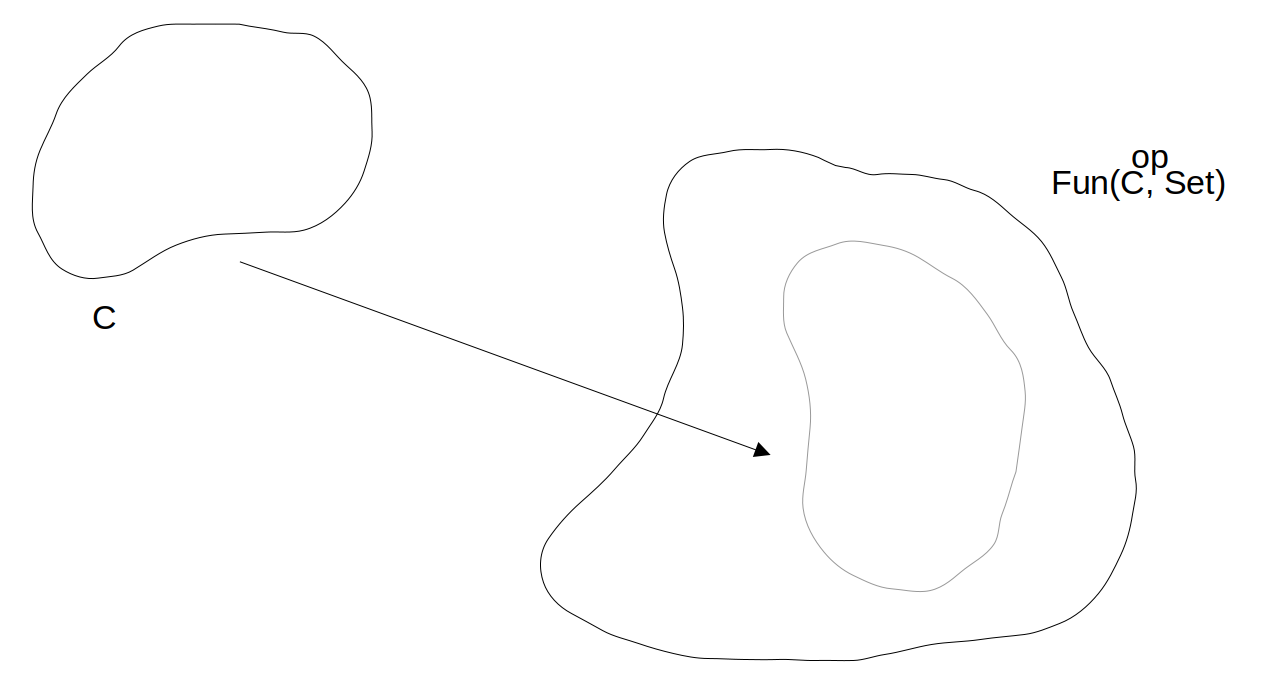
\includegraphics[width=1\textwidth]{emb.png}
\end{figure}

\noindent
où la flèche représente le foncteur de Yoneda/l'intégration de Yoneda. Plus précisément, $Y:\mathcal C\to\textbf{Fun}(\mathcal C^\text{op}, \textbf{Set})$ est un foncteur \textit{covariant} qui part de la catégorie $\mathcal C$ pour arriver à la catégorie des foncteurs \textit{contravariants} à valeurs dans \textbf{Set}.

\subsubsection{Le lemme de Yoneda}
L'intégration de Yoneda abordée précédemment peut être sujette à deux points de vues : soit il s'agit d'un corollaire du lemme de Yoneda, soit d'un cas particulier qui nous permet de le décrire. Nous avons adopté le second point de vue, il nous reste alors à énoncer ce lemme :\\

\begin{lemma}[Lemme de Yoneda]{}
    Soit $\mathcal C$ une catégorie (localement petite). Pour tout objet $C\in\mathcal C$ et pour tout foncteur $F\in\textbf{Fun}(\mathcal C^\text{op}, \textbf{Set})$, il existe un unique isomorphisme $$\Hom(Y(C), F)\cong F(C)$$ qui est, de plus, naturel en $F$ et en $C$.
\end{lemma}

\noindent
Dans cet énoncé,

\begin{itemize}[label=\textbullet]
    \item $Y(C)$ est l'intégration de Yoneda.
    \item $\Hom$ est $\Hom_{\textbf{Fun}(\mathcal C^\text{op}, \textbf{Set})}$.
    \item "Naturel en $F$" signifie que, pour $\mathfrak G:F\to G$, on a
    \begin{center}
    \begin{tikzcd}
    {\Hom(Y(C), F)} \arrow[rr, "\cong"] \arrow[dd, "{\Hom(Y(C), \mathfrak G)}"] &  & F(C) \arrow[dd, "\mathfrak G"] \\
                                                                                &  &                                \\
    {\Hom(Y(C), G)} \arrow[rr, "\cong"]                                         &  & G(C)                          
    \end{tikzcd}
    \end{center}
    \item "Naturel en $C$" signifie que, pour $h:C\to D$, on a
    \begin{center}
    \begin{tikzcd}
    {\Hom(Y(C), F)} \arrow[rr, "\cong"] \arrow[dd, "{\Hom(Y(h), F)}"] &  & F(C) \arrow[dd, "F(h)"] \\
                                                                      &  &                         \\
    {\Hom(Y(D), F)} \arrow[rr, "\cong"]                               &  & F(D)                   
    \end{tikzcd}
    \end{center}
\end{itemize}

En d'autres termes, le lemme de Yoneda suggère qu'au lieu d'étudier la catégorie $\mathcal C$, il est possible d'étudier la catégorie de tout les foncteurs $\mathcal C\to\textbf{Set}$. Ce lemme est important car, de façon analogue au théorème de Cayley, l'étude des objets et des morphismes dans la catégorie des ensembles est souvent bien plus simple que dans la catégorie $\mathcal C$ d'origine.

\begin{proof}[Lemme de Yoneda]{}
    La preuve est laissée en exercice au lecteur.
\end{proof}

\subsubsection{Application du lemme de Yoneda}
Pour résumer, le lemme de Yoneda dit que l'on peut obtenir un objet $X$ à un isomorphisme près à partir de la connaissance des foncteurs hom-set $\Hom(Y, X)$ pour tout autre objet $Y$. Quelles sont les applications de ce lemme ? Le lemme de Yoneda est souvent utilisé dans des applications qui prennent la forme suivante : étant donné deux objets $A, B\in\mathcal C$, si on veut montrer que $A\cong B$ alors il suffit de montrer que $Y(A)\cong Y(B)$ dans $\textbf{Fun}(\mathcal C^\text{op}, \textbf{Set})$. Il vient alors le corollaire :

\begin{lemma}[Principe de Yoneda]{}
    Soient $A$ et $B$ des objets d'une catégorie $\mathcal C$ localement petite, alors
    $$
    Y(A)\cong Y(B)\ \implies\ A\cong B.
    $$
\end{lemma}

Il est en effet plus facile de donner un morphisme $Y(A)\to Y(B)$ qu'un morphisme $A\to B$, la catégorie $\textbf{Fun}(\mathcal C^\text{op}, \textbf{Set})$ possédant beaucoup de structures et propriétés qui sont familières.\\

Donnons un exemple illustrant le lemme de Yoneda au travers de catégories qui nous sont plutôt familières.

\begin{example}[]{}
    Soit \textbf{Set} et soient $A, B\in\text{Ob}(\textbf{Set})$. Nous voulons montrer que, dans cette catégorie, il existe un isomorphisme naturel entre l'ensemble $\{f:A\to B\}$ et l'ensemble $\{g:B^A\to B\}$, où $B^A\defeq\{h:A\to B\}$. Pour se faire, nous allons utiliser le lemme de Yoneda. Fixons un "ensemble test" $C$ et montrons qu'il existe un isomorphisme naturel entre les fonctions $C\to B^A$ et les fonctions $C\to B$.\\

    \noindent
    Considérons le foncteur $\Hom(\emd, A)$ qui envoie chaque ensemble $X$ sur l'ensemble des fonctions $\Hom(X, A)$ et chaque fonction $f:X\to Y$ sur la fonction $\Hom(f, A):\Hom(Y, A)\to\Hom(X, A)$. Le lemme de Yoneda affirme qu'il existe un isomorphisme naturel entre les fonctions $C\to B^A$ et les transformations naturelles $\eta:\Hom(\emd, A)\to\Hom(\emd, B)$ avec la composante $\eta_C:\Hom(C, A)\to\Hom(C, B)$. Pour chaque fonction $g:C\to B^A$, on définit la transformation naturelle $\eta^g$ par $\eta^g_X(f)\defeq g\circ f$ pour tout $X$ et toute fonction $f:X\to A$. Alors, pour chaque $f:C\to A$, nous avons que $\eta^g_C(f)=g\circ f$, et donc $\eta^g_C=g$.\\

    \noindent
    Aussi, pour chaque transformation naturelle $\eta:\Hom(\emd, A)\to\Hom(\emd, B)$ avec $\eta_C:\Hom(C, A)\to\Hom(C, B)$, on définit la fonction $g_\eta:C\to B^A$ par $g_{\eta(c)}(a)\defeq\eta_{C(c)}(a)$ pour tout $c$ dans $C$ et tout $a$ dans $A$. Alors, pour chaque $f:C\to A$, nous avons que $g_\eta\circ f=\eta_C(f)$, et donc $g_\eta=\eta_C$.\\

    \noindent
    Cela montre qu'il existe bien un isomorphisme naturel entre les deux ensembles, de plus, dans le cas de \textbf{Set}, cet isomorphisme naturel est une bijection naturelle. $\blacksquare$
\end{example}

\newpage
\section{Conclusion}
Pendant cette semaine de stage, j'ai acquis les bases de la théorie des catégories. J'ai appris ce que sont les catégories, comment les construire et décrire des objets et des morphismes spécifiques tels que les monomorphismes, les épimorphismes, les objets initiaux et terminaux. J'ai également exploré les foncteurs, qui sont des "mappings" entre les catégories, en particulier le foncteur hom-set. J'ai appris que les transformations naturelles permettent d'effectuer des "mappings" de ces foncteurs. J'ai également exploré les propriétés universelles (UMP) en étudiant différents exemples. Enfin, j'ai découvert le lemme de Yoneda, ainsi que ses applications et conséquences.\\

Malheureusement, durant le stage, je n'ai pas eu l'occasion d'apprendre et/ou de pratiquer tout ce qui a été initialement proposé, de plus les concepts qui sont arrivés plus tardivement durant la semaine, comme le lemme de Yoneda, n'ont pas eu le temps d'être profondément explorés, je n'en retire donc que d'assez brèves connaissances.

\section{Bibliographie}
Plusieurs ressources ont été utilisés durant ce stage. Tout ce que j'ai expliqué dans ce rapport est issue de ma compréhension du sujet, ainsi que des divers notes et exercices que j'ai réalisés durant le stage et l'encadrement avec le promoteur. Les ressources utilisées sont les suivantes :

\begin{itemize}
    \item Awodey, Steve. Category Theory, second edition. New York, Oxford University Press, 2010.
    \item Milewski Bartosz. Category Theory for Programmers. Open access Book, 2017.
    \item Mac Lane, Saunders. Categories for the Working Mathematicia, second edition. New York, Springer, 1998.
    \item Riehl, Emily. Category theory in context. Cambridge, Cambridge University Press, 2014.
    \item Hassani, Sadri. Mathematical Physics, second edition. New York, Springer, 2013.
    \item Coecke, Bob. Introducing categories to the pratcticing physicist.
\end{itemize}

\sectionline
\end{document}
